\chapter{Molybdenum dichalcogenides as cathodes for rechargeable AIBs} % Main chapter title
In this chapter, we discuss performance of AIBs using two-dimensional molybdenum dichalcogenides such as \ce{MoS2}, \ce{MoSe2} and MoSSe in their bulk and nano form, as cathodes for AIBs attempt to establish their mechanism.
\label{chap4} % For referencing the chapter elsewhere, use \ref{Chapter1} 

%Many successful battery electrodes are based on 2D-layered materials. We have studied aluminium-ion batteries using molybdenum dichalcogenides --- \ce{MoS2}, \ce{MoSe2} and MoSSe as active cathode materials. The batteries showed clear discharge voltage plateaus in the ranges 1.6 - 1.4 V for \ce{MoS2} and \ce{MoSe2}, and 0.6 - 0.5 V for MoSSe. \ce{MoS2} and \ce{MoSe2} have similar crystal structures, interestingly we found that \ce{MoSe2} performed better than MoS2. MoSSe exhibited a higher specific capacity over \ce{MoS2} and \ce{MoSe2}, but the energy density was lower than \ce{MoSe2} at a current density of 40 mA g$^-{^1}$, \ce{MoSe2} proved to be more stable with a discharge specific capacity of 110 mAh g$^-{^1}$ with an average potential at $\sim 2.0 V$. The cell was stable at 100 mA g$^-{^1}$ for over 200 cycles with 90 \% coulombic efficiency. 

\section{Theory and background}
Transition metal dichalcogenides (TMDs) have a strong in-plane covalent bonding and weaker vdW bonds exist between any two layers, which is quite similar to graphene layers in graphite. The 2D structure facilitates intercalation of ions within these layers. Molybdenum dichalcogenides not only provide redox variability but also a high theoretical capacity (600-1200 mAh g$^{-1}$). The intercalation voltage observed with \ce{MX2}, where M = Mo, W, Ti, etc. and X = S and Se, is high ($\approx$ 2.0 V). The mechanism that TMDs follow is based on intercalation as well as conversion. 
We explored different molybdenum dichalcogenide-based cathodes and their mechanism of energy storage. We expected that two-dimensional (2D) layered materials that support intercalation of charged species might be suitable as active cathode materials in AIBs. Molybdenum dichalcogenides (\ce{MoX2}) display similar properties as graphite. Amongst various transition metal chalcogenides, \ce{MoS2} has been extensively used as a cathode for rechargeable batteries \cite{li_rechargeable_2018-2, zhu_fast_2015-2}. These materials have a layered structure, which allows intercalation of ions and they are electrically conductive. The intra-layer spacing between \ce{MoS2} is at around 6.5 \AA, which can easily accommodate any volumetric expansion on cycling \cite{liang_rechargeable_2011,hu_ws2_2013}. These properties make them attractive candidates for AIB cathodes. In 2015, Geng \textit{et al.} found that \ce{Al^{3+}} ions fully intercalated into chevrel phase \ce{Mo6S8} with the cations occupying two different sites in the crystal lattice \cite{geng_reversible_2015}. The discharging and charging reactions were proposed as follows:
\begin{align*}
          \ce{Al + 7AlCl4^- &<-> 4Al2Cl7^- + 3e^-}\\
\ce{8AlCl7^- + 6e^- + Mo6S8 &<-> Al2Mo6S8 + 14AlCl4^-}
\end{align*}
Three years later, Li \textit{et al.} prepared \ce{MoS2} microspheres by a simple hydrothermal method \cite{li_rechargeable_2018-2}. They proposed a similar mechanism where \ce{Al^{3+}} ions inserted into the electrode accompanied by a phase transformation at the electrode interface. It has been reported that transition metal dichalcogenide electrodes tend to transition from a 2H phase into a more conducting 1T phase when used in a battery \cite{fan_hybrid_2017}. Li and his group confirmed this phase-transition by using \textit{ex-situ} XPS and XRD etching techniques. The reaction equations for this battery system were proposed as follows:
\begin{align*}
    \ce{MoS2 + x\ce{Al3+}  + 3x\ce{e-} &<-> Al_xMoS2}\\
    \ce{xAl + 7x\ce{AlCl4-} &<-> 4x\ce{Al2Cl7-} + 3x\ce{e-}}
\end{align*}
In general, these cells showed a relatively low energy density and had reversibility issues in the redox processes.
We studied a range of 2D molybdenum dichalcogenides including \ce{MoS2}, \ce{MoSe2} and \ce{MoSSe}, and tested them as cathodes for non-aqueous AIBs. Our unpublished, preliminary density functional theory (DFT) calculations indicated a significant decrease in inter-layer spacing of these materials when \ce{Al^{3+}} cations were assumed to intercalate (owing to the very high charge density of \ce{Al^{3+}}). Therefore, we propose intercalation of \ce{AlCl4-} anions into the layered cathode. XRD, Raman spectroscopy and XPS were used to verify our hypothesis. Surprisingly we found that \ce{MoSe2}-based cathodes performed different and better than all of the other molybdenum dichalcogenides.
\section{Experimental methods}
Same as discussed in Chapter 3.
\section{Results and Discussion}
Figures \ref{Figures/chap4fig:crys} displays the crystal structure of \ce{MoX2} where X is sulfur (S) and/or selenium (Se). The material has two vacant sites for intercalation - M1 and M2. M1 denotes the spaces in between the X-Mo-X atoms (Figure \ref{Figures/chap4fig:crys}b) whereas M2 represents the space created by separation of two layers of \ce{MoX2} with an inter-layer distance of 6.3 $\AA$ (Figure \ref{Figures/chap4fig:crys}c). The layers are held together by van der Waals (vdW) forces. M2 presents an open network and provides various interstitial sites, which can easily accommodate the \ce{AlCl4-} anions, which are 5.28 $\AA$ in size as reported by Takahashi {\it et al} \cite{takahashi_niv2o5nh2o_2005}. Our preliminary results showed that \ce{Al^{3+}} would \lq contract\rq\ the \ce{MoX2} layers when trying to intercalate, making \ce{AlCl4-} anion intercalation more likely. Also, the triply charged \ce{Al^{3+}} cation has to overcome strong electrostatic force from the \ce{S^{2-}} or \ce{Se^{2-}} anion network in order to enter \ce{MoX2} layers. Moreover, participation of the cation is limited due to its tendency to form strong bonds with the chalcogenides making the intercalation/deintercalation process slow and irreversible. Therefore, we propose intercalation of \ce{AlCl4-} anions from the electrolyte into M2 sites of \ce{MoX2} when the cells charge. Galvanostatic cycles, cyclic voltammetry (CV) scans, XRD, Raman and XPS results discussed later, strongly support our claim of a reversible intercalation process especially taking place in  \ce{MoSe2}. 
\begin{figure}[htb!]
\centering
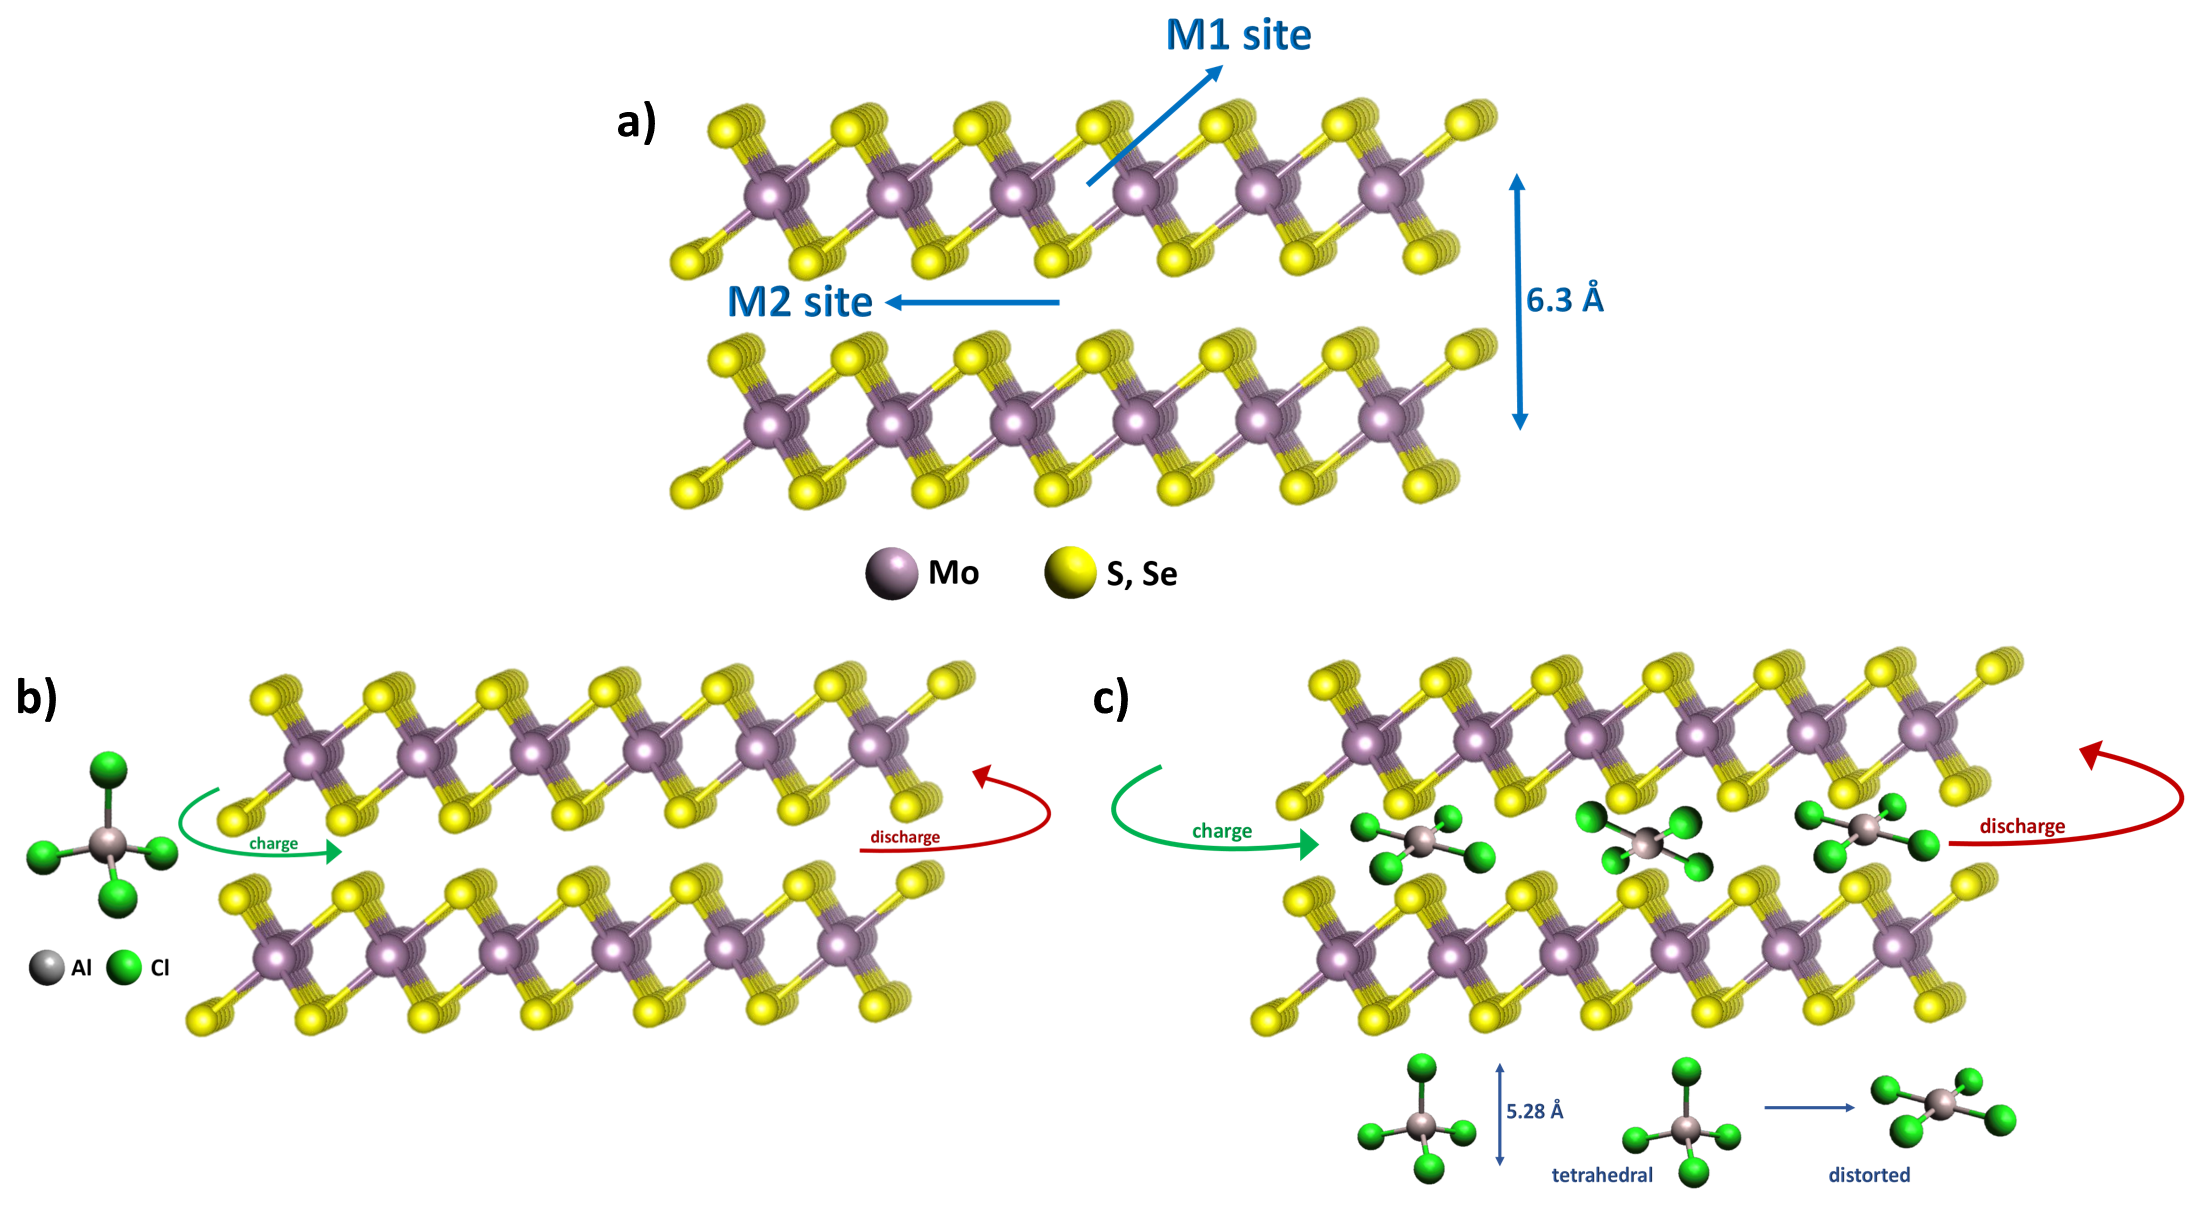
\includegraphics[width=\textwidth]{Figures/chap4fig/crys}
\caption{Schematic representation of a) an MoX$_2$ crystal structure with possible intercalation sites at M1 and M2 b) intercalation at M1 site and c) intercalation at M2 site.}
 \label{Figures/chap4fig:crys}
\end{figure}
 \begin{figure}[htb!]
\centering
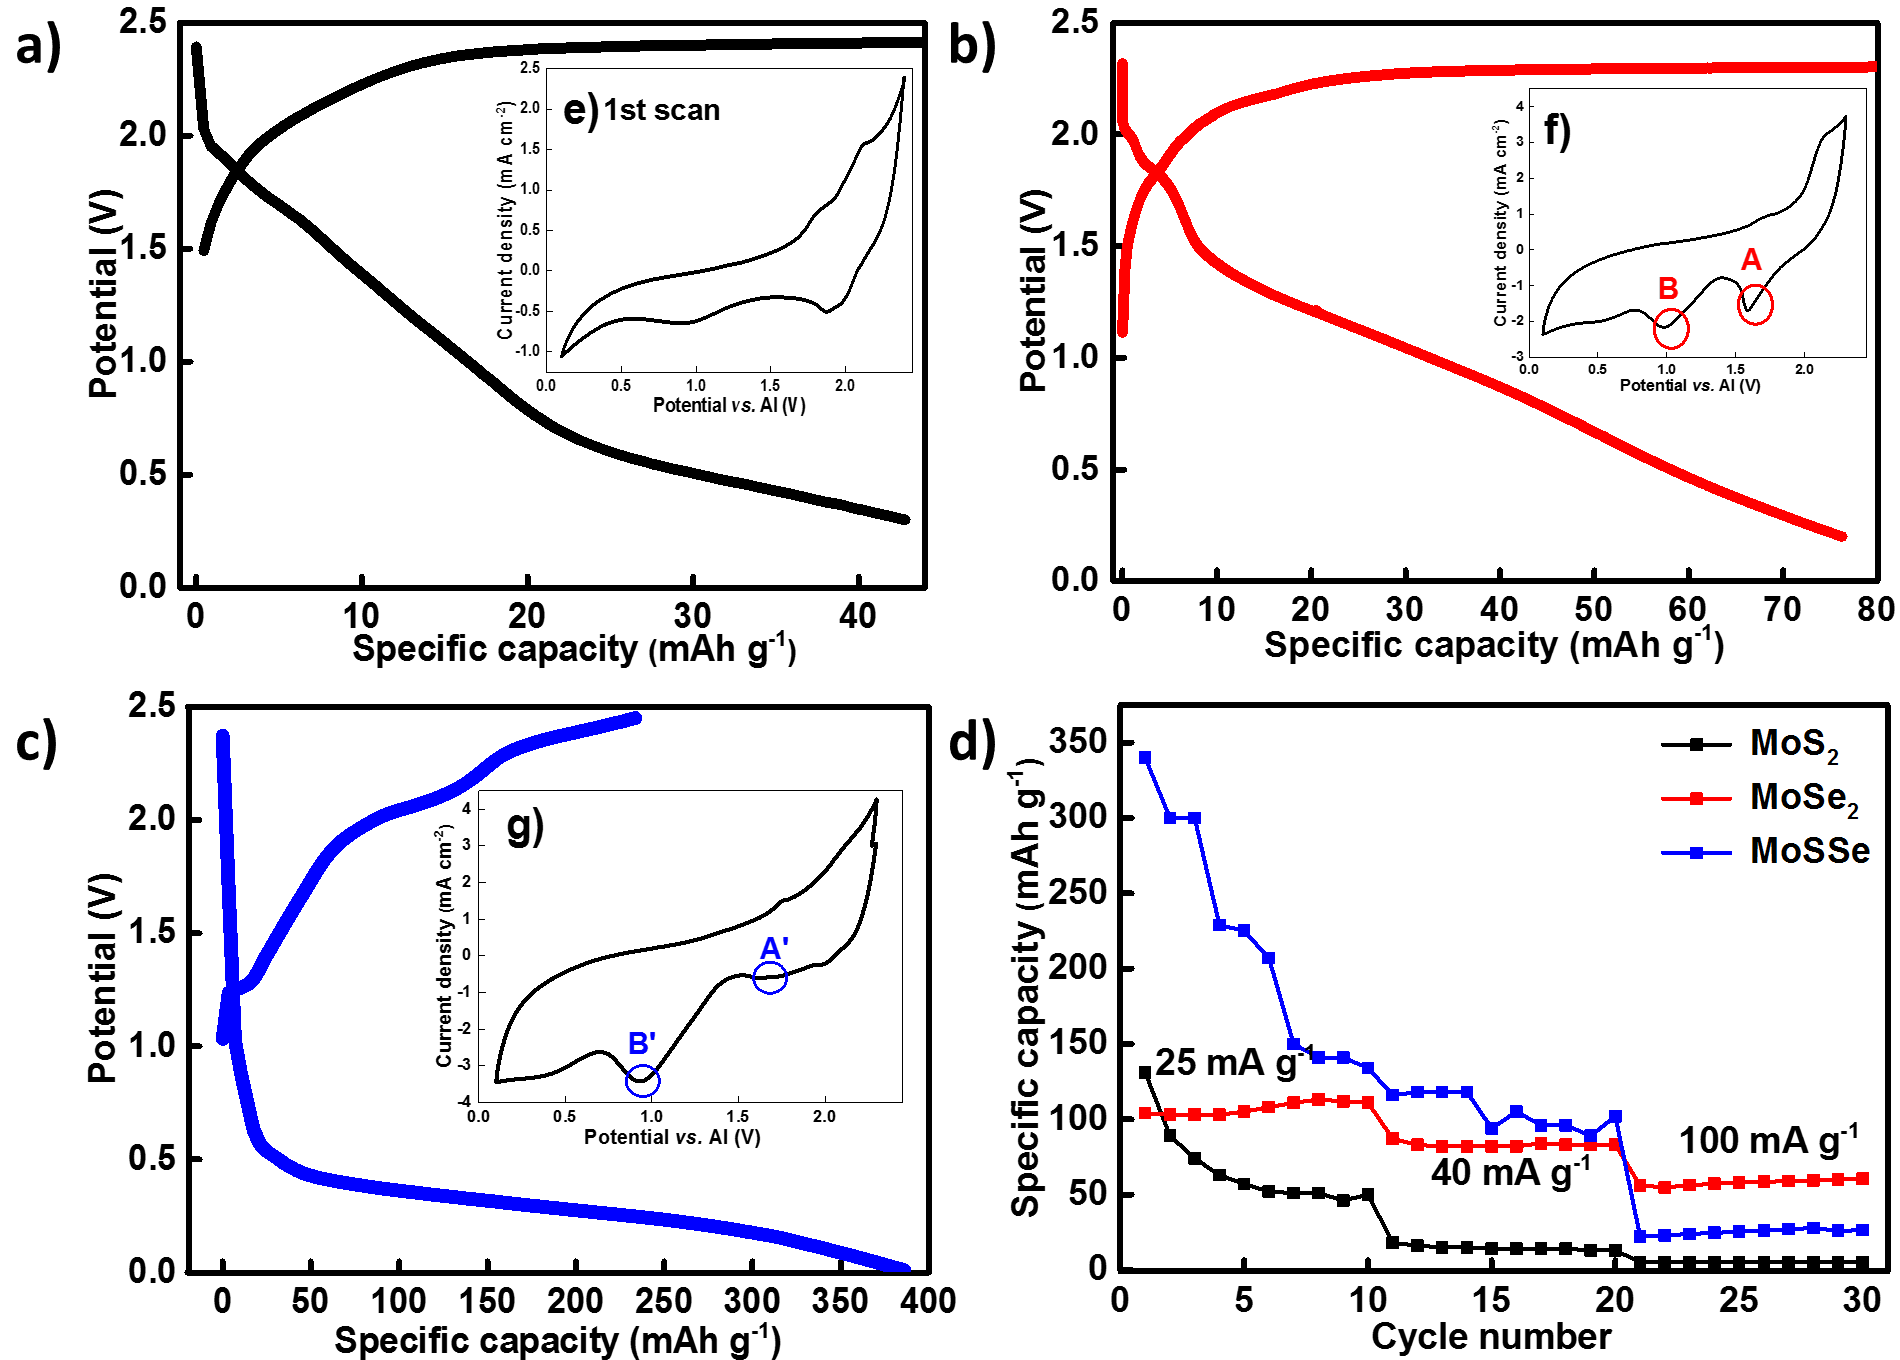
\includegraphics[width=\textwidth]{Figures/chap4fig/CDCCV}
\caption{First charge/discharge curve at 40 mA g$^{-1}$ for a) \ce{MoS2}, b) \ce{MoSe2} and c) MoSSe. d) Specific capacities of \ce{MoS2}, \ce{MoSe2} and MoSSe at current rates of 25, 40 and 100 mA g$^{-1}$. e)First CV scan of \ce{MoS2}, f) \ce{MoSe2} and g) MoSSe at a scan rate of 10 mV s$^{-1}$ in an aluminium-ion battery against Al reference electrode.}
\label{Figures/chap4fig:CDCCV}
\end{figure} 
A modified two-electrode polyether ether ketone (PEEK) cell was used for conducting preliminary electrochemical tests. Electrode preparations and cell configurations are described in the Experimental Methods section. We found that \ce{MoSe2} was superior to \ce{MoS2} and MoSSe. Voltage plateaus in the CDCs matched well with the peaks observed in their respective CV scans. MoSSe was relatively unstable with poor coulombic efficiency of $\sim$50\%. Specific capacity for Al/MoSSe cell decreased rapidly and the cells became inactive after 20-25 cycles. We hypothesise that Se substitution in \ce{MoS2} was non-uniform, which is why the material does not have a uniform crystal structure. Therefore, intercalation of \ce{AlCl4-} degraded our cathode structure after every cycle and reduced the cell efficiency.
Figure \ref{Figures/chap4fig:CDCCV} shows the charge-discharge curves (CDCs) for \ce{MoS2} (Figure \ref{Figures/chap4fig:CDCCV}a), \ce{MoSe2} (Figure \ref{Figures/chap4fig:CDCCV}b) and MoSSe (Figure \ref{Figures/chap4fig:CDCCV}c). Discharge voltages plateaus/bends  were observed at 1.8 V and 0.6 V  for \ce{MoS2}, 1.9 V, 1.7 V  and 1.5 V for \ce{MoSe2} and 0.5 V for MoSSe. Al/ \ce{MoS2} recorded its first discharge capacity at 43 mAh g$^{-1}$, which reduced to 40 mAh g$^{-1}$ and 31 mAh g$^{-1}$ in its second and third cycle respectively (Figure\ref{Figures/chap4fig:S1}a). We compared its first cycle with the first CV scan (Figure \ref{Figures/chap4fig:CDCCV}e) and found a good resemblance between the discharge voltage plateau and reduction peak positions, and in between the charging plateau and oxidation peak positions. Initial CDCs of the Al/\ce{MoSe2} cell revealed some interesting results. With discharge plateaus at 1.9 V and 1.7 V, its first CV scan showed a reduction peak at 1.65 V (point A in Figure\ \ref{Figures/chap4fig:CDCCV}b) and another one at 1.0 V (point B). The peak at 1.0 V suggested an irreversible reaction (this peak was absent in the following scans), which can be attributed to an irreversible phase transition that is known to take place in molybdenum dichalcogenides \cite{fan_hybrid_2017}. During this transition, a semi-conducting 2H phase converts into a more metallic 1T phase.  This transition increased the interlayer spacing of \ce{MoSe2} (by reducing the vdW forces) and allowed more \ce{AlCl4-} ions to intercalate. From Figure \ref{Figures/chap4fig:mose2}, it is clear that the redox processes are reversible even after 200 cycles  at a higher current rate of 100 mAg$^{-1}$. Al/MoSSe cell observed three distinct plateaus during charge at 1.7 V, 2.0 V and 2.3 V in its first cycle with a discharge plateau at 0.5 V. The presence of various charging potentials might correspond to multiple oxidation processes that might occur due to individual interaction of \ce{AlCl4-} with S and Se atoms. 
\begin{figure}[htb!]
\centering
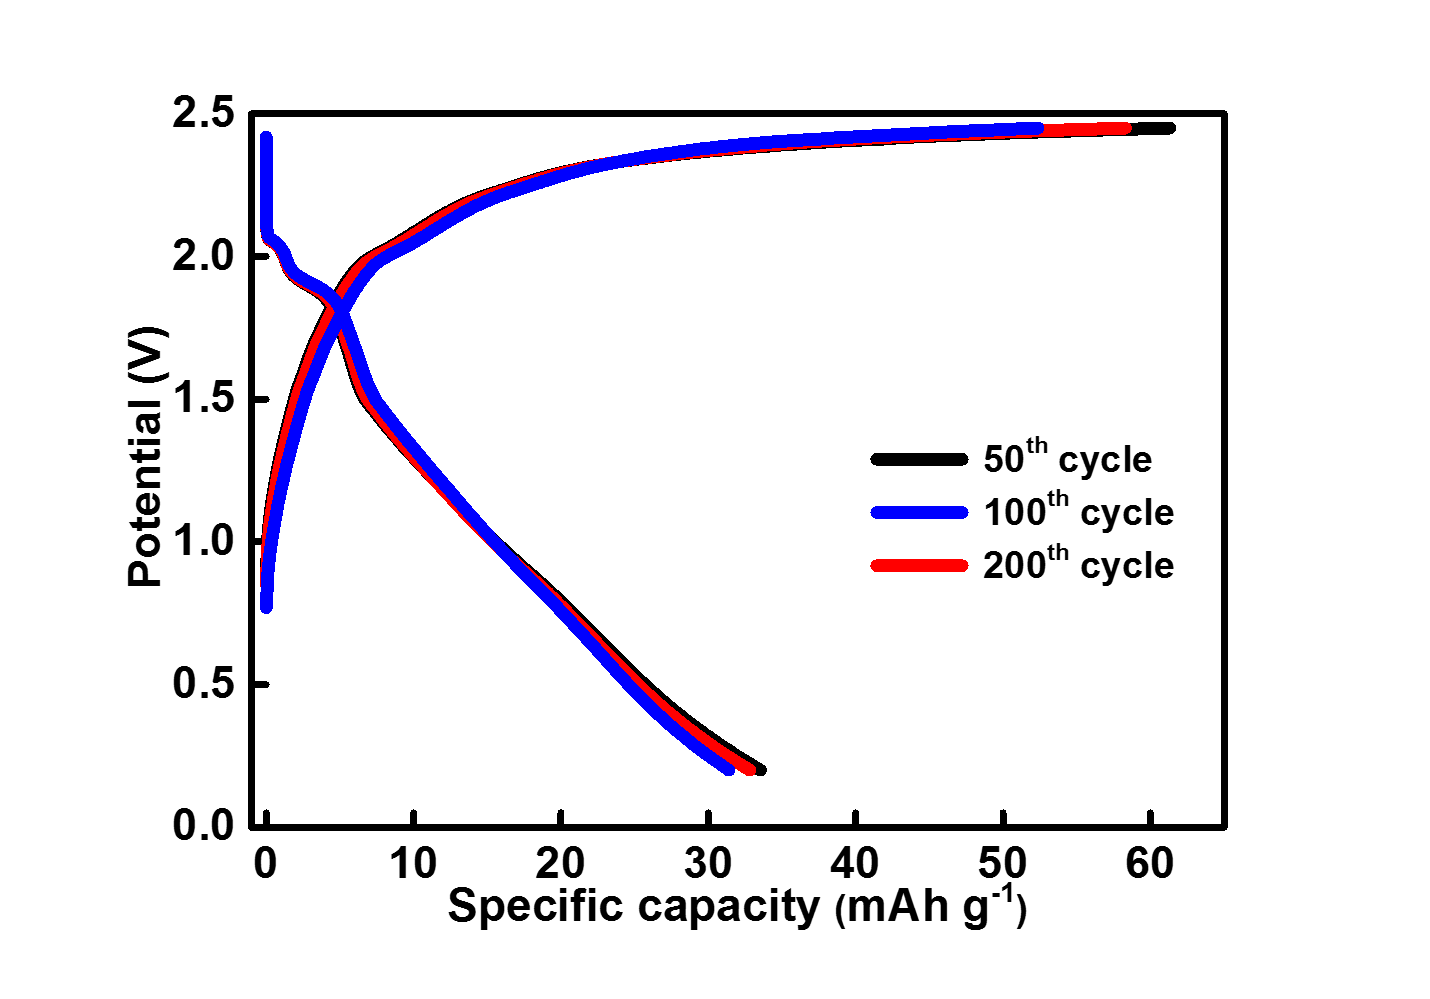
\includegraphics[width=\textwidth]{Figures/chap4fig/mose2}
\caption{Long-term cycle life of \ce{MoSe2} when charged and discharged to 2.45 V and 0.2 V against \ce{Al^{3+}}/Al anode. Cell capacity was retained after 200 cycles at a current rate of 100 mA g$^{-1}$.}
\label{Figures/chap4fig:mose2}
\end{figure}
The first CV scan, Figure \ref{Figures/chap4fig:CDCCV}c revealed an irreversible reduction potential at 0.9 V, point B', like \ce{MoSe2}, implying a similar phase transition. Only one reduction peak at 1.7 V (point A') was noted in the consecutive scans with decreased intensity after every cycle. However, no plateau was observed in the CDC at that potential. Further investigation is required for MoSSe as no clear trend could be observed. Results were recorded at different current rates (25, 40 and 100 mA g$^{-1}$) for the three electrodes in Figure \ref{Figures/chap4fig:CDCCV}d. \ce{MoSe2}, recorded the most stable capacities at all potentials compared to \ce{MoS2} (lowest capacity of 11 at 100 mA/g) and MoSSe with a significant drop in capacity after every cycle at all current rates. 
\begin{figure}[htb!]
\centering
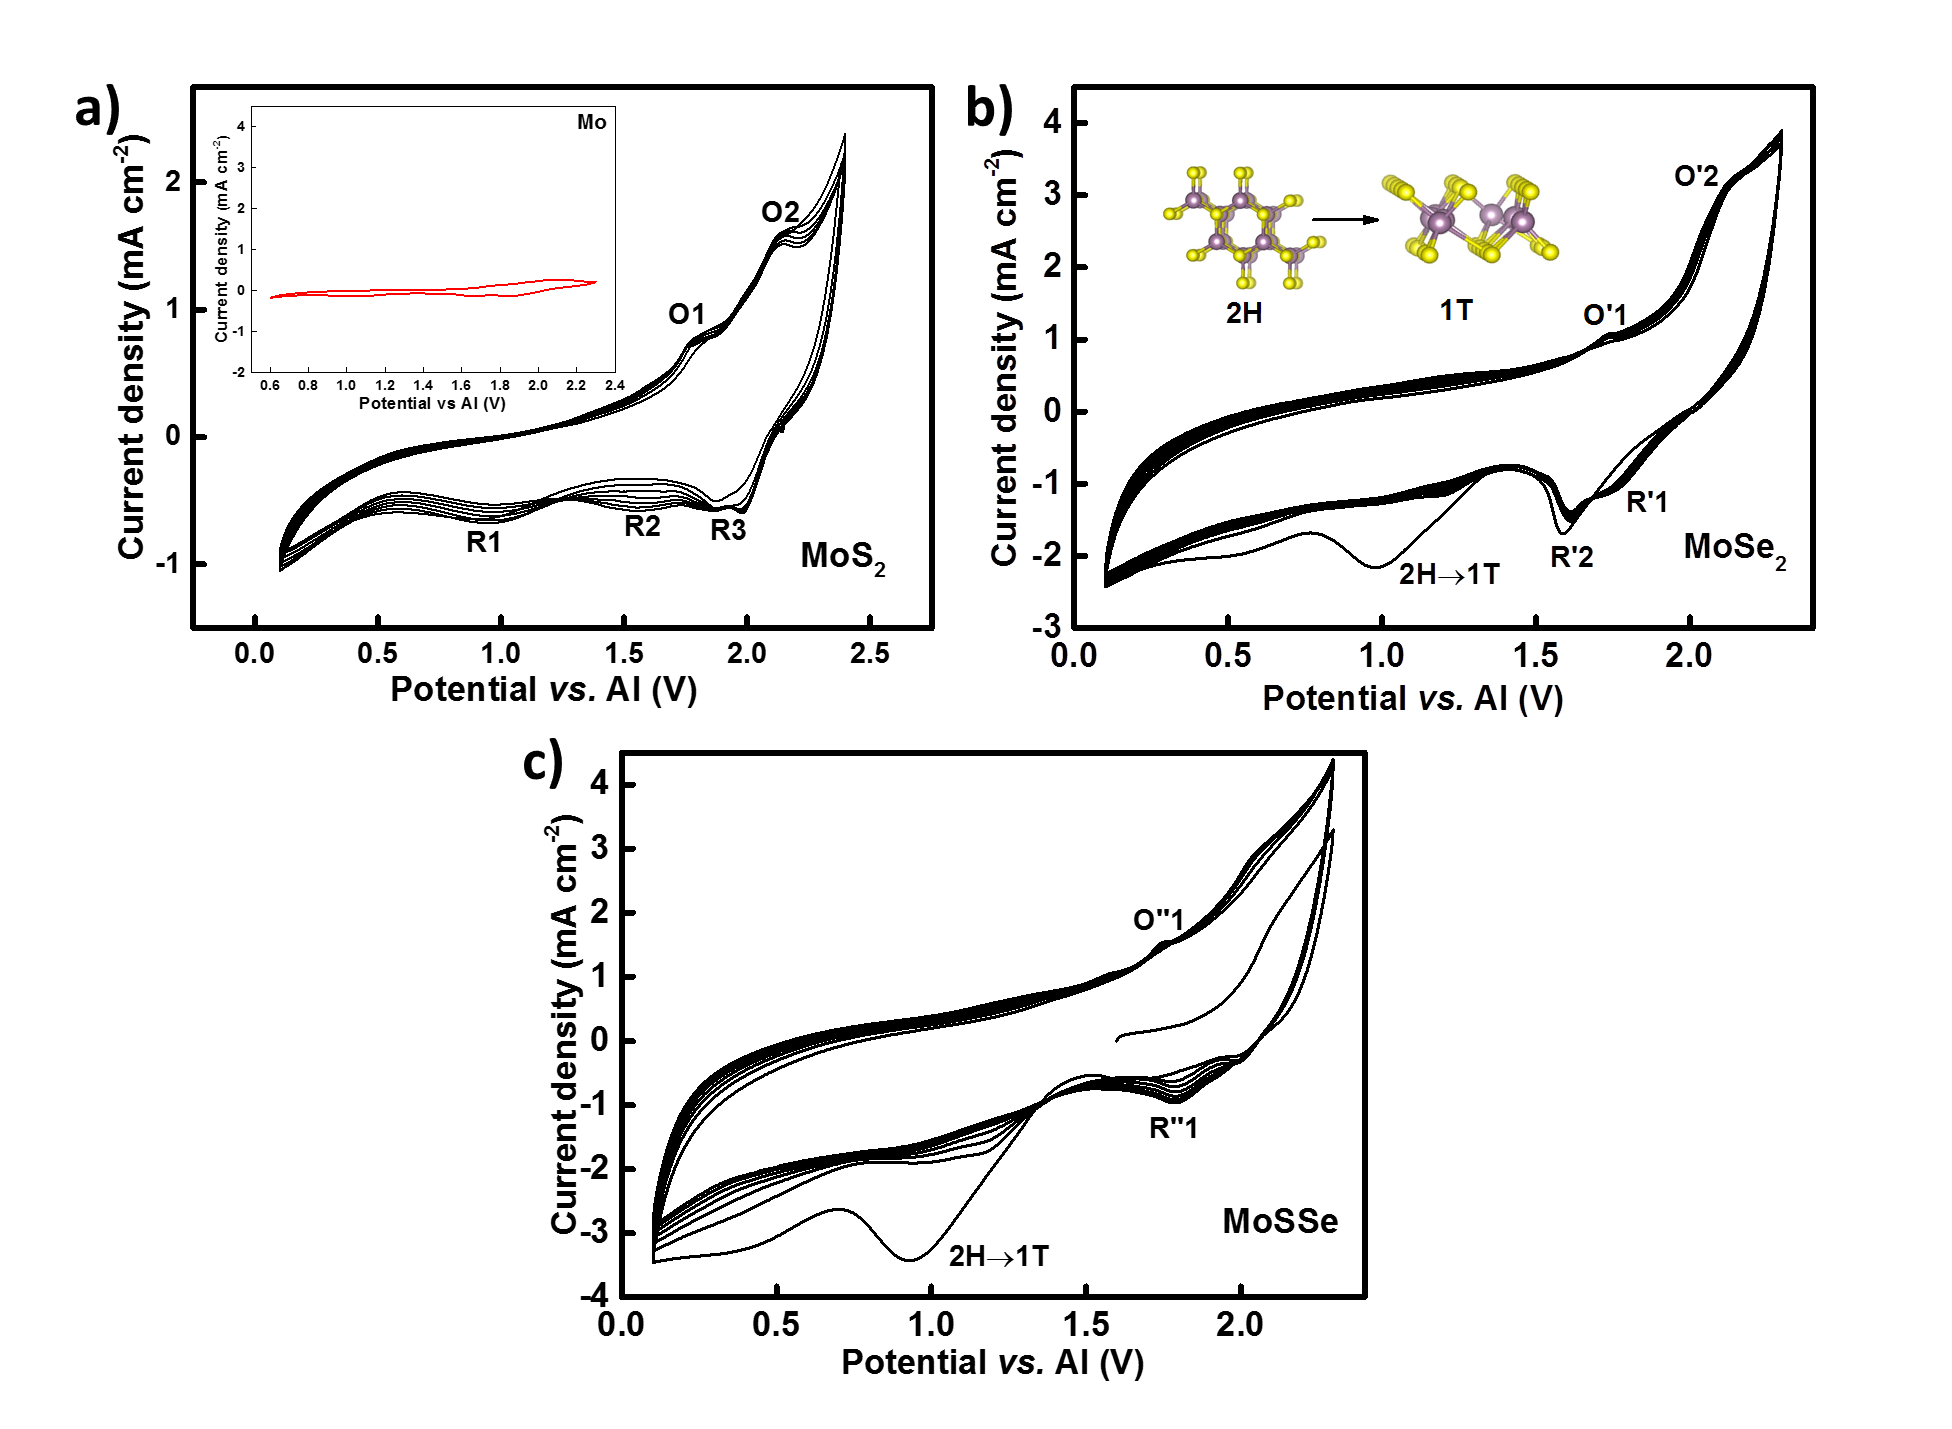
\includegraphics[width=\textwidth]{Figures/chap4fig/CV}
\caption{Cyclic voltammetric scans of a) \ce{MoS2}, b) \ce{MoSe2} and c) MoSSe at a scan rate of 10 mV s$^{-1}$ in a two-electrode aluminium-ion cell against an Al reference electrode.}
\label{Figures/chap4fig:CV}
\end{figure} 

Both \ce{MoS2} and \ce{MoSe2} have similar interlayer distance (6.3 \AA) but \ce{MoSe2} showed a higher capacity and a more stable cycle life than \ce{MoS2}. To account for this behaviour, we compared the CV scans of all electrodes at a scan rate of 10 mV/s$^{-1}$ in Figure \ref{Figures/chap4fig:CV}. Different charge storage mechanisms can lead to different CV curves. Capacitors have a rectangular CV curve whereas batteries show oxidation and reduction peaks in their CVs \cite{jiao_aluminum-ion_2016}. Firstly, we noted that CVs of \ce{MoSe2} and MoSSe in Figure \ref{Figures/chap4fig:CV}b and c respectively, covered a higher area than \ce{MoS2} (Figure \ref{Figures/chap4fig:CV}a). This suggested an additional electrostatic charge-storage mechanism taking place. In addition, the phase transition for \ce{MoSe2} and MoSSe (2H$\rightarrow$1T) was prominent in their first scan at approx. 0.9 V. No such transitions were observed for \ce{MoS2}. Charge storage in \ce{MoS2} is primarily based on reversible oxidation and reduction of Mo in \ce{MoS2} (from \ce{Mo^{4+}} to \ce{Mo^{5+}}) with the oxidation peaks observed at 1.8 (O1) and 2.1 V (O2), and corresponding reduction peak at 2.0 V (R3). The presence of two more reduction peaks at 1.6V (R2) and 0.9 V (R1), with their peak intensities decreasing after every scan showed adsorption/desorption of \ce{AlCl4-} onto the electrode. Al/\ce{MoSe2} cell in Figure \ref{Figures/chap4fig:CV}b indicated an intercalation/deintercalation process and a capacitor-like charge storage. With the following scans coinciding with each other, two oxidation peaks at 1.7 V (O'1) and 2.1 V (O'2) and corresponding reduction peaks at 1.8 V (R'1) and 1.6 V (R'2) were observed suggesting a highly reversible electrochemical reaction. CV scans of MoSSe lacked evidence for a reversible redox process. With one oxidation peak at 1.7 V (O''1) and a reduction peak at 1.8 V who's intensity increased after every scan (R''1), it was difficult to conclude whether the cell's capacity approx. 250\ce{mAh g^{-1}} was derived from faradaic reactions or simply electrostatic intercalation on the cathode surface. CV curve from Mo foil (Figure\ \ref{Figures/chap4fig:CV}a inlet) proved that the current collector did not give a capacitance of its own.
\begin{figure}[htb!]
\centering
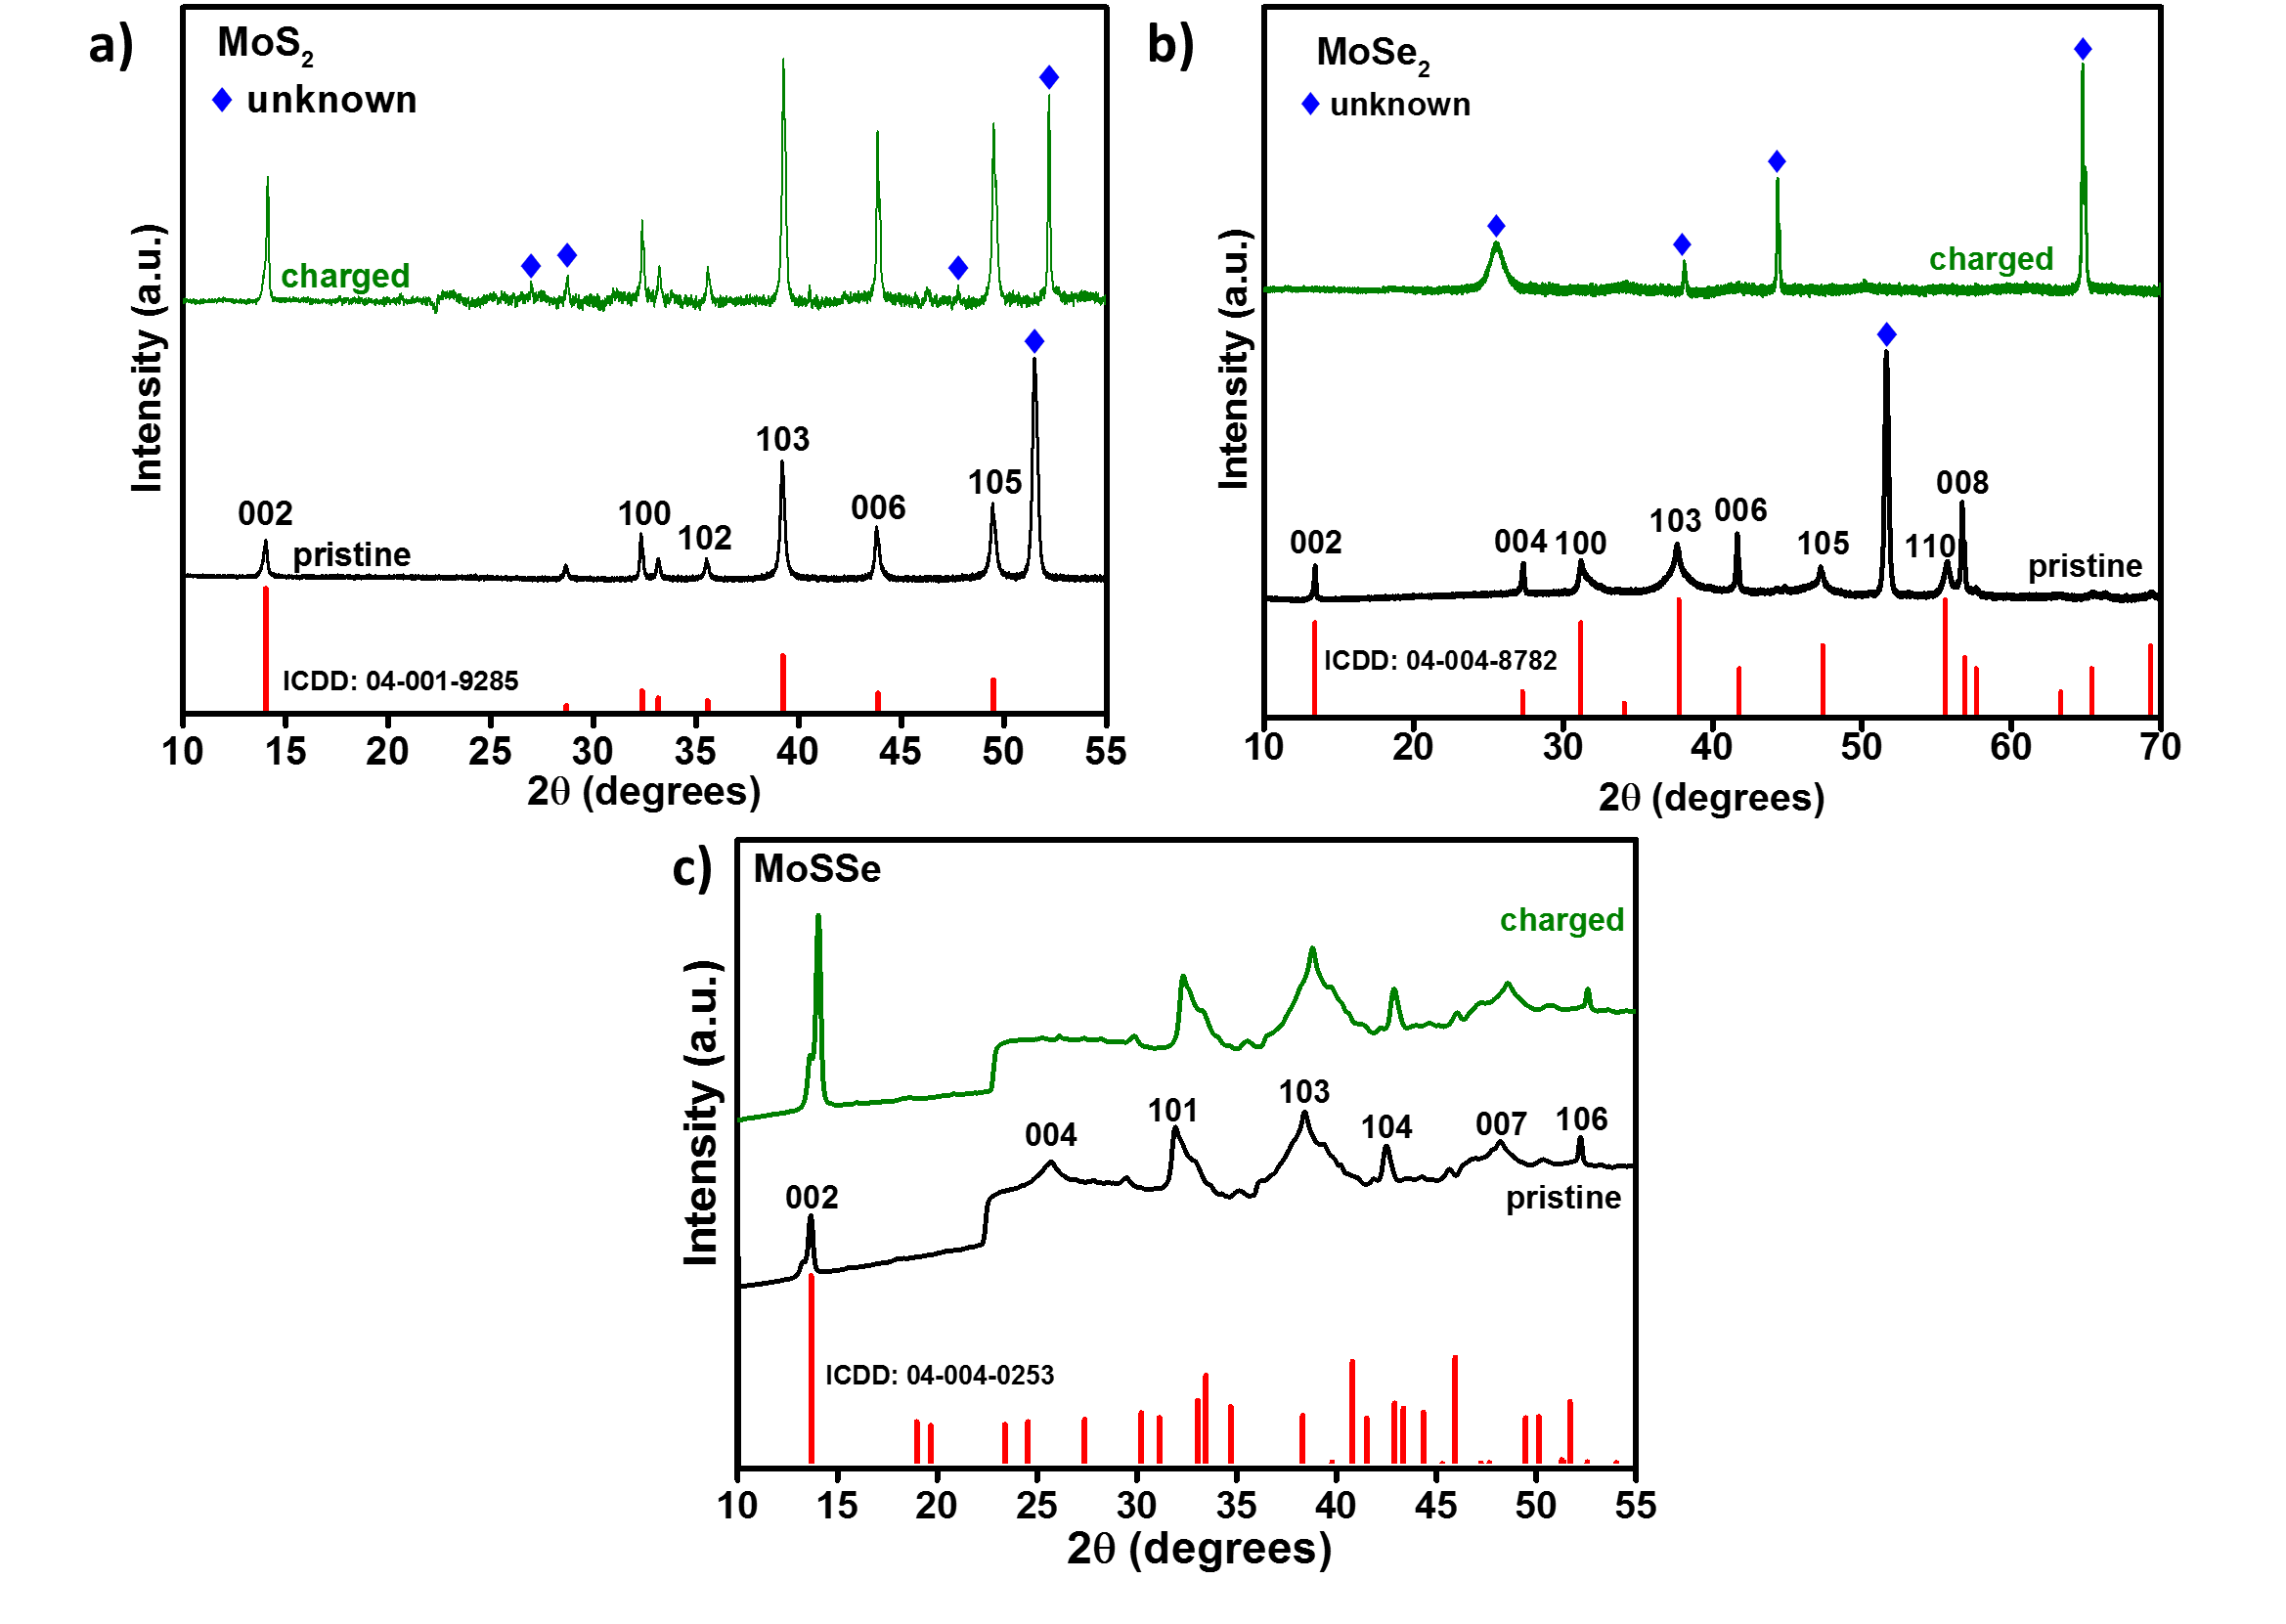
\includegraphics[width=\textwidth]{Figures/chap4fig/XRD}
\caption{X-ray diffraction (XRD) spectra of pristine (black) and charged (green) a) \ce{MoS2}, b) \ce{MoSe2} and c) MoSSe electrodes charged to 2.35 V and discharged to 0.2 V vs. \ce{Al3+}/Al, with International Centre for Diffraction Data (ICDD) references (in red) for pristine cathodes.}
\label{Figures/chap4fig:XRD}
\end{figure}
Figure \ref{Figures/chap4fig:XRD} displays the XRD spectra of \ce{MoS2}, \ce{MoSe2} and MoSSe electrodes. Since it has been found that intercalation occurs when the cells are charging, we compared the charged electrodes with the pristine ones. Figure \ref{Figures/chap4fig:XRD}a shows the pristine (in black) and charged electrode (in green) of an Al/\ce{MoS2} cell. It was observed that the 002 plane shifted from 14.21$^\circ$ to 14.02$^\circ$ suggesting a very small increase in the inter-layer distance of the layered material. An amorphous nature of the charged electrode was expected as the cell was cycled 20 times, which might have resulted in a less ordered structure. Most of the peaks in \ce{MoS2} retained their positions. \ce{MoSe2} (Figure\ \ref{Figures/chap4fig:XRD}b) on the other hand, displayed significantly shifted peaks after charge. The diffraction peak at 13.4$^\circ$ (002) disappeared after charging, whereas the peaks at 27.28$^\circ$ (004), 41.64$^\circ$ (006) and 51.59$^\circ$ (106) shifted to 25.58$^\circ$ , 38.08$^\circ$  and 44.38$^\circ$ respectively. A decrease in theta values of 004 and 006 planes (along the c-axis of the crystal lattice) indicated an increase in the inter-layer spacing. These observations support our hypothesis of \ce{AlCl4-} intercalation during charge. It was interesting to note that MoSSe, however, did not have a well-defined crystal structure to begin with, as was evident from its pristine electrode in Figure \ref{Figures/chap4fig:XRD}c (in black). Since no increase in inter-layer spacing was observed despite a high specific capacity (Figure\ \ref{Figures/chap4fig:S1}c), it was confirmed that the capacity for this material comes from a non-faradaic reaction,  where ions electrostatically absorb onto the surface of electrode. 


To confirm the intercalation of \ce{AlCl4-} in \ce{MoSe2} we used XPS, which is a useful tool for distinguishing various oxidation states and helps in identifying different polymorphs (2H and 1T) \cite{fan_hybrid_2017}. The detailed narrow spectrum scans in Figure \ref{Figures/chap4fig:XPS} display the binding energy of Mo (3d$_{5/2}$ and 3d$_{3/2}$) and Al 2p peaks for charged \ce{MoSe2} and MoSSe electrodes. For pristine \ce{MoSe2}, molybdenum showed two peaks at 229.1 eV and 232.2 eV corresponding to 3d$_{5/2}$ and 3d$_{3/2}$ (Figure\ \ref{Figures/chap4fig:S3}a). Selenium displayed a doublet at 55.4 eV and 54.6 eV corresponding to Se 3d$_{3/2}$ and 3d$_{5/2}$ respectively (Figure\ \ref{Figures/chap4fig:S4}a). Peak splitting in an XPS spectrum indicates a phase change or a change in oxidation state. Consequently, the peak for Mo 3d split into three doublets indicating \ce{Mo^{4+}}, \ce{Mo^{5+}} and \ce{Mo^{6+}} (Figure\ \ref{Figures/chap4fig:XPS}a). Se 3d observed one broad peak, which deconvoluted into four peaks after the cells were charged in the \ce{MoSe2} cell, Figure\ \ref{Figures/chap4fig:S4}b. Pristine electrodes of MoSSe contained Mo in more than one oxidation state and suggested the presence of both polymorphs (2H and 1T) in Figure\ \ref{Figures/chap4fig:S3}b. After the cells were charged, the peak areas increased for Mo at 231.7 eV (3d$_{5/2}$) and 228.6 eV (3d$_{3/2}$), Figure\ \ref{Figures/chap4fig:XPS}b. Conversion to the 1T phase can be seen with an increase in the area of the 1T polymorph \cite{fan_hybrid_2017}. In addition, Se 3d observed one broad peak, which deconvoluted into four peaks after the cells were charged in MoSSe cell, Figure\ \ref{Figures/chap4fig:S4}c and d. A new peak at ~236 eV in Mo 3d spectra for \ce{MoS2}, \ce{MoSe2} and MoSSe electrodes corresponded to Mo$^{6+}$ species due to formation of \ce{MoO3} after the electrode was exposed in air. Overall, oxidation states of Mo change only for charged \ce{MoS2} and \ce{MoSe2} cathodes. This signifies that MoSSe does not undergo any redox reaction and the capacity is mainly derived from a surface-based adsorption of anions. As expected, charged electrodes showed higher concentration of aluminium and chlorine than discharged electrodes in Figure\ \ref{Figures/chap4fig:S5}a and b. 
\begin{figure}[htb!]
\centering
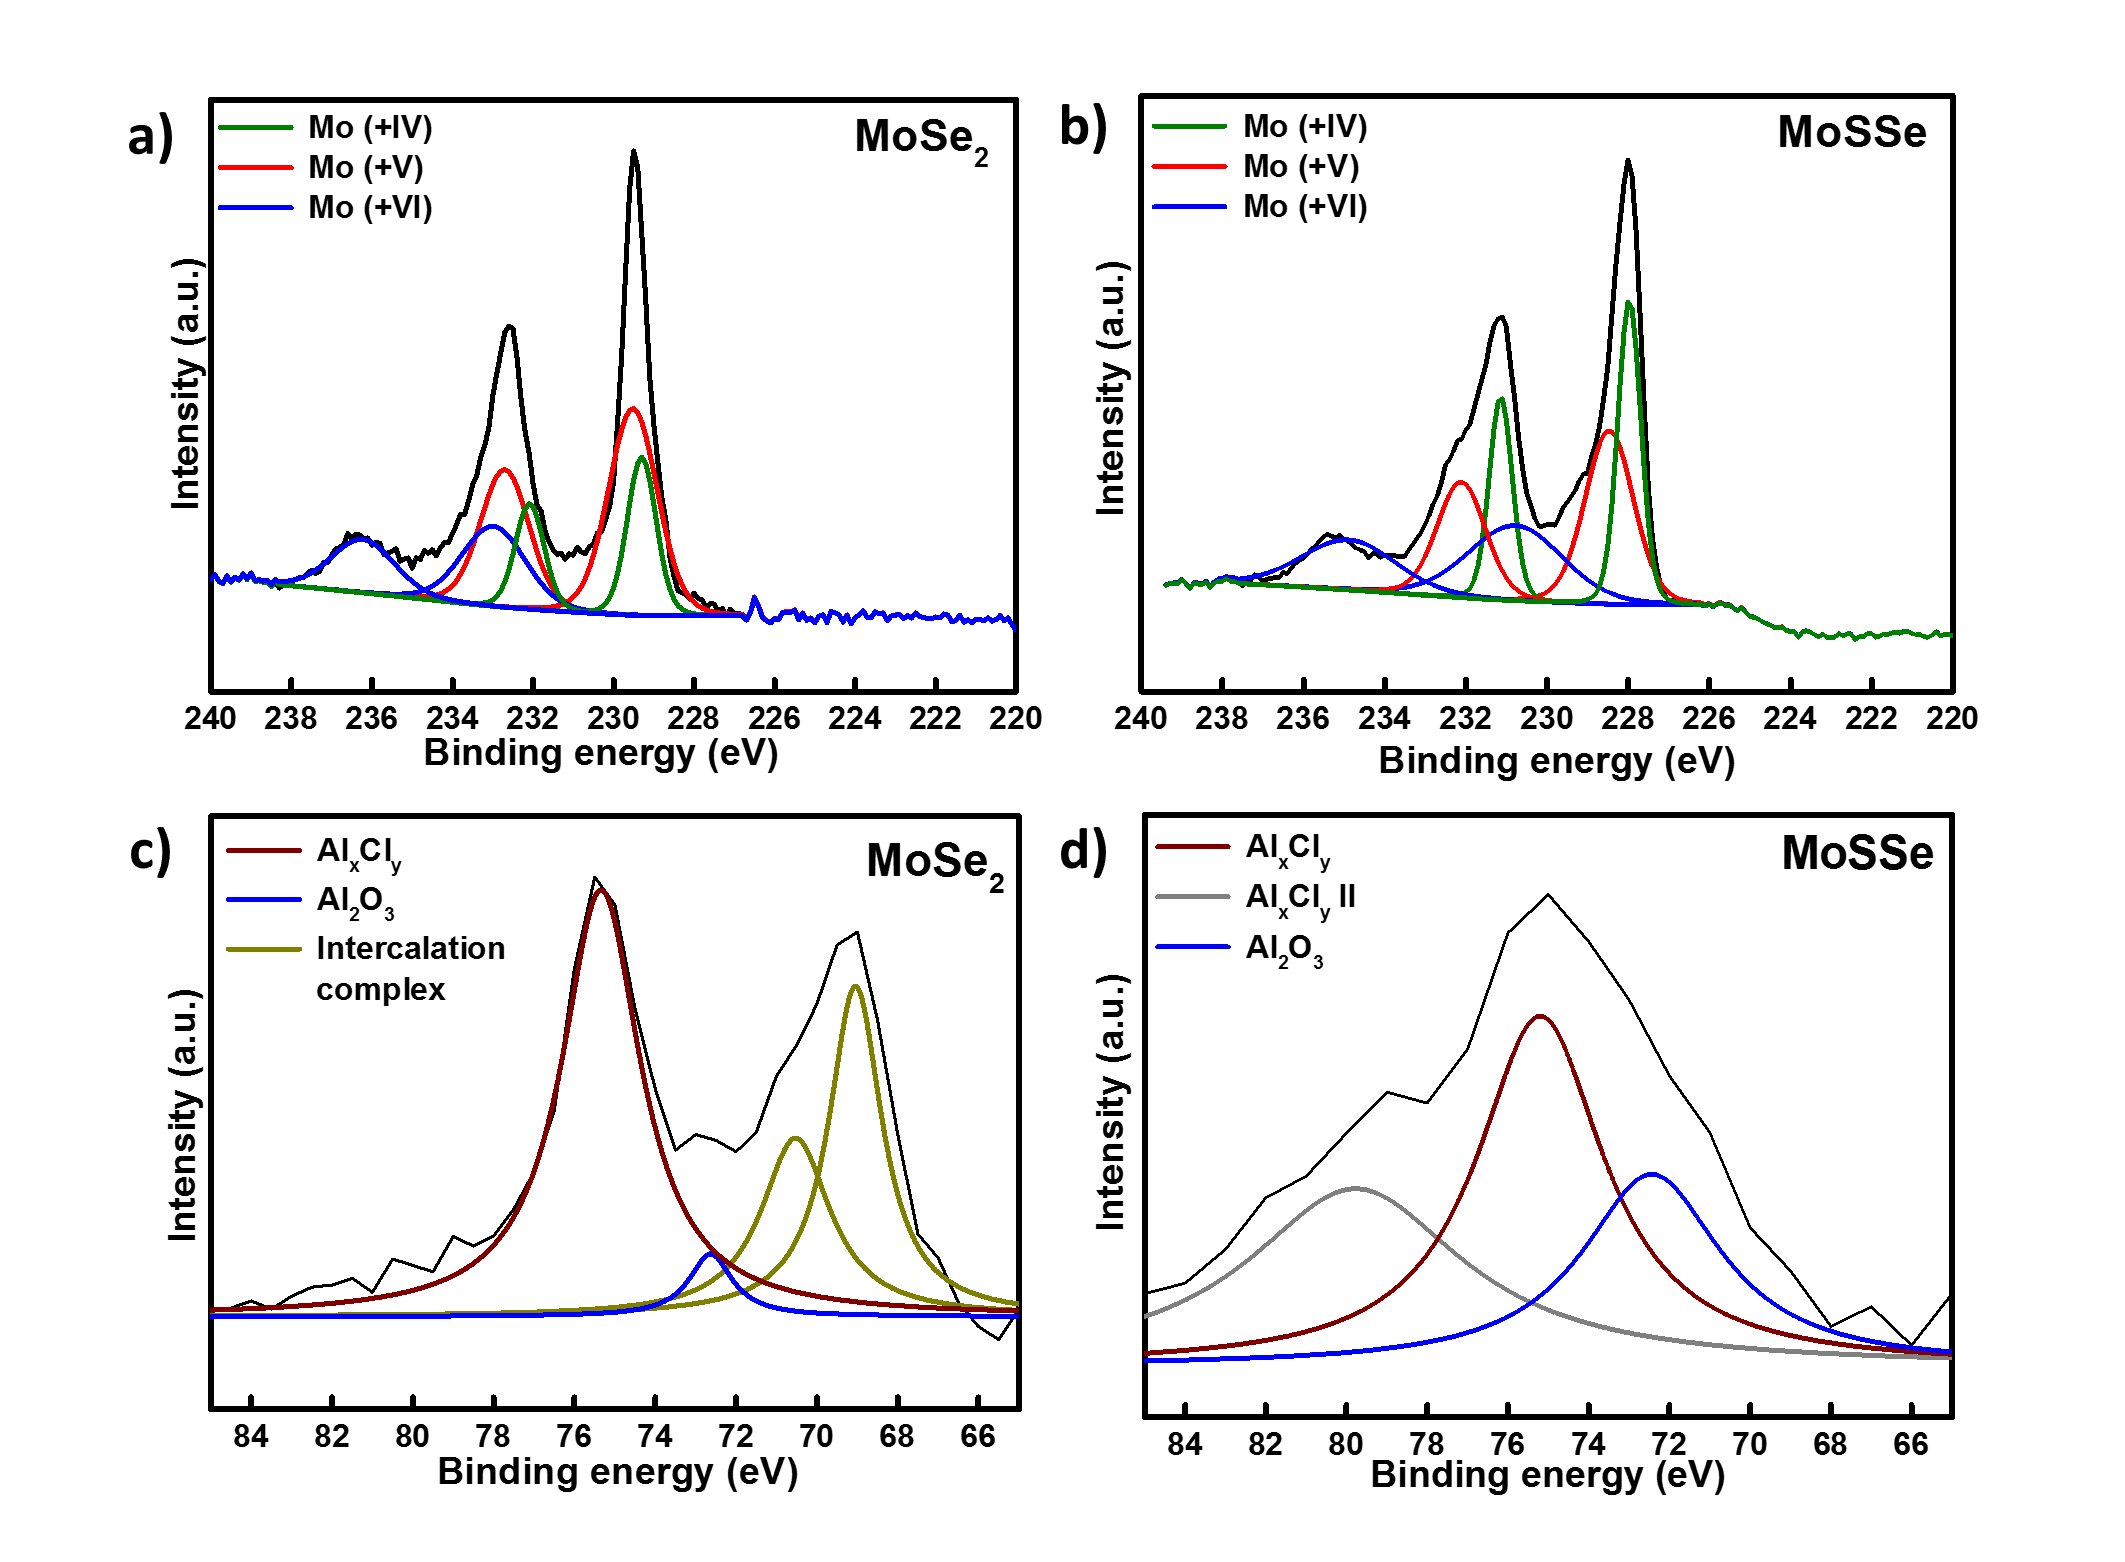
\includegraphics[width=\textwidth]{Figures/chap4fig/XPS}
\caption{XPS spectra of Mo 3d orbital in a charged a) \ce{MoSe2} and b) MoSSe cathode and Al 2p orbital in a charged c) \ce{MoSe2} and d) MoSSe cathode.}
\label{Figures/chap4fig:XPS}
\end{figure}

Charged \ce{MoSe2} electrodes displayed binding energies of Al 2p at 77 eV (in red) and 76 eV (in blue) corresponding to chlorides (\ce{AlxCly}) and \ce{Al2O3} respectively in Figure \ref{Figures/chap4fig:XPS}c. A new peak at 69 eV (in green) was detected. This peak can be assigned to a new complex formed after \ce{AlCl4-} intercalation. The data strongly suggests insertion of \ce{AlCl4-} in \ce{MoSe2} and formation of a new complex that changes the oxidation state of both Mo and Al. An overall spectra of charged \ce{MoS2}, \ce{MoSe2} and MoSSe cathodes is shown in Figure\ \ref{Figures/chap4fig:S6}.

In addition we compared the Raman spectra of pristine and charged electrodes to detect shifts in vibrational modes of the lattice, Figure \ref{Figures/chap4fig:raman}. E$^1_{2g}$ and A$^1_g$ are the most intense vibrational modes for molybdenum dichalcogenides \cite{yang_pressure-induced_2019, r_2d_2017,sharma_stable_2018}. Peaks corresponding to E$^1_{2g}$ and A$^1_g$ modes for \ce{MoS2} (Figure \ref{Figures/chap4fig:raman}a) are prominent at 384.6 cm$^{-1}$ and 410.2 cm$^{-1}$ respectively. A$^1_g$ indicates an out-of-plane symmetric displacement of S atoms, whereas E$^1_{2g}$ suggests an in-layer displacement. Also, separation between the two indicates a multi-layer structure, which was observed for all three materials. No significant peak shift or peak broadening was observed for the charged \ce{MoS2} electrode. For 2H\ce{MoSe2} (Fig.\ \ref{Figures/chap4fig:raman}b), A$^1_g$ is the most intense vibration occurring at a frequency lower than that of E$^1_{2g}$. When the number of layers decreases, the A$^1_g$ mode softens (increase in full-width-at-half-maximum (FWHM)). Spectra generated after intercalation were different from the pristine cathodes because phase conversion from 2H to 1T decreases the molecule's symmetry and more Raman bands get active. The presence of J1 and J2 peaks in addition to E$^1_{2g}$ and A$^1_g$ at lower wavelengths suggest the existence of 1T phase especially for \ce{MoSe2} and MoSSe (inset, Figure\ \ref{Figures/chap4fig:raman}b and c). This agrees with our CV scans where a phase transition was observed for \ce{MoSe2} and MoSSe. Raman results confirm our XRD results suggesting chloroalumination reduced the symmetry of \ce{MoSe2}'s crystal lattice. 
\begin{figure}[htb!]
\centering
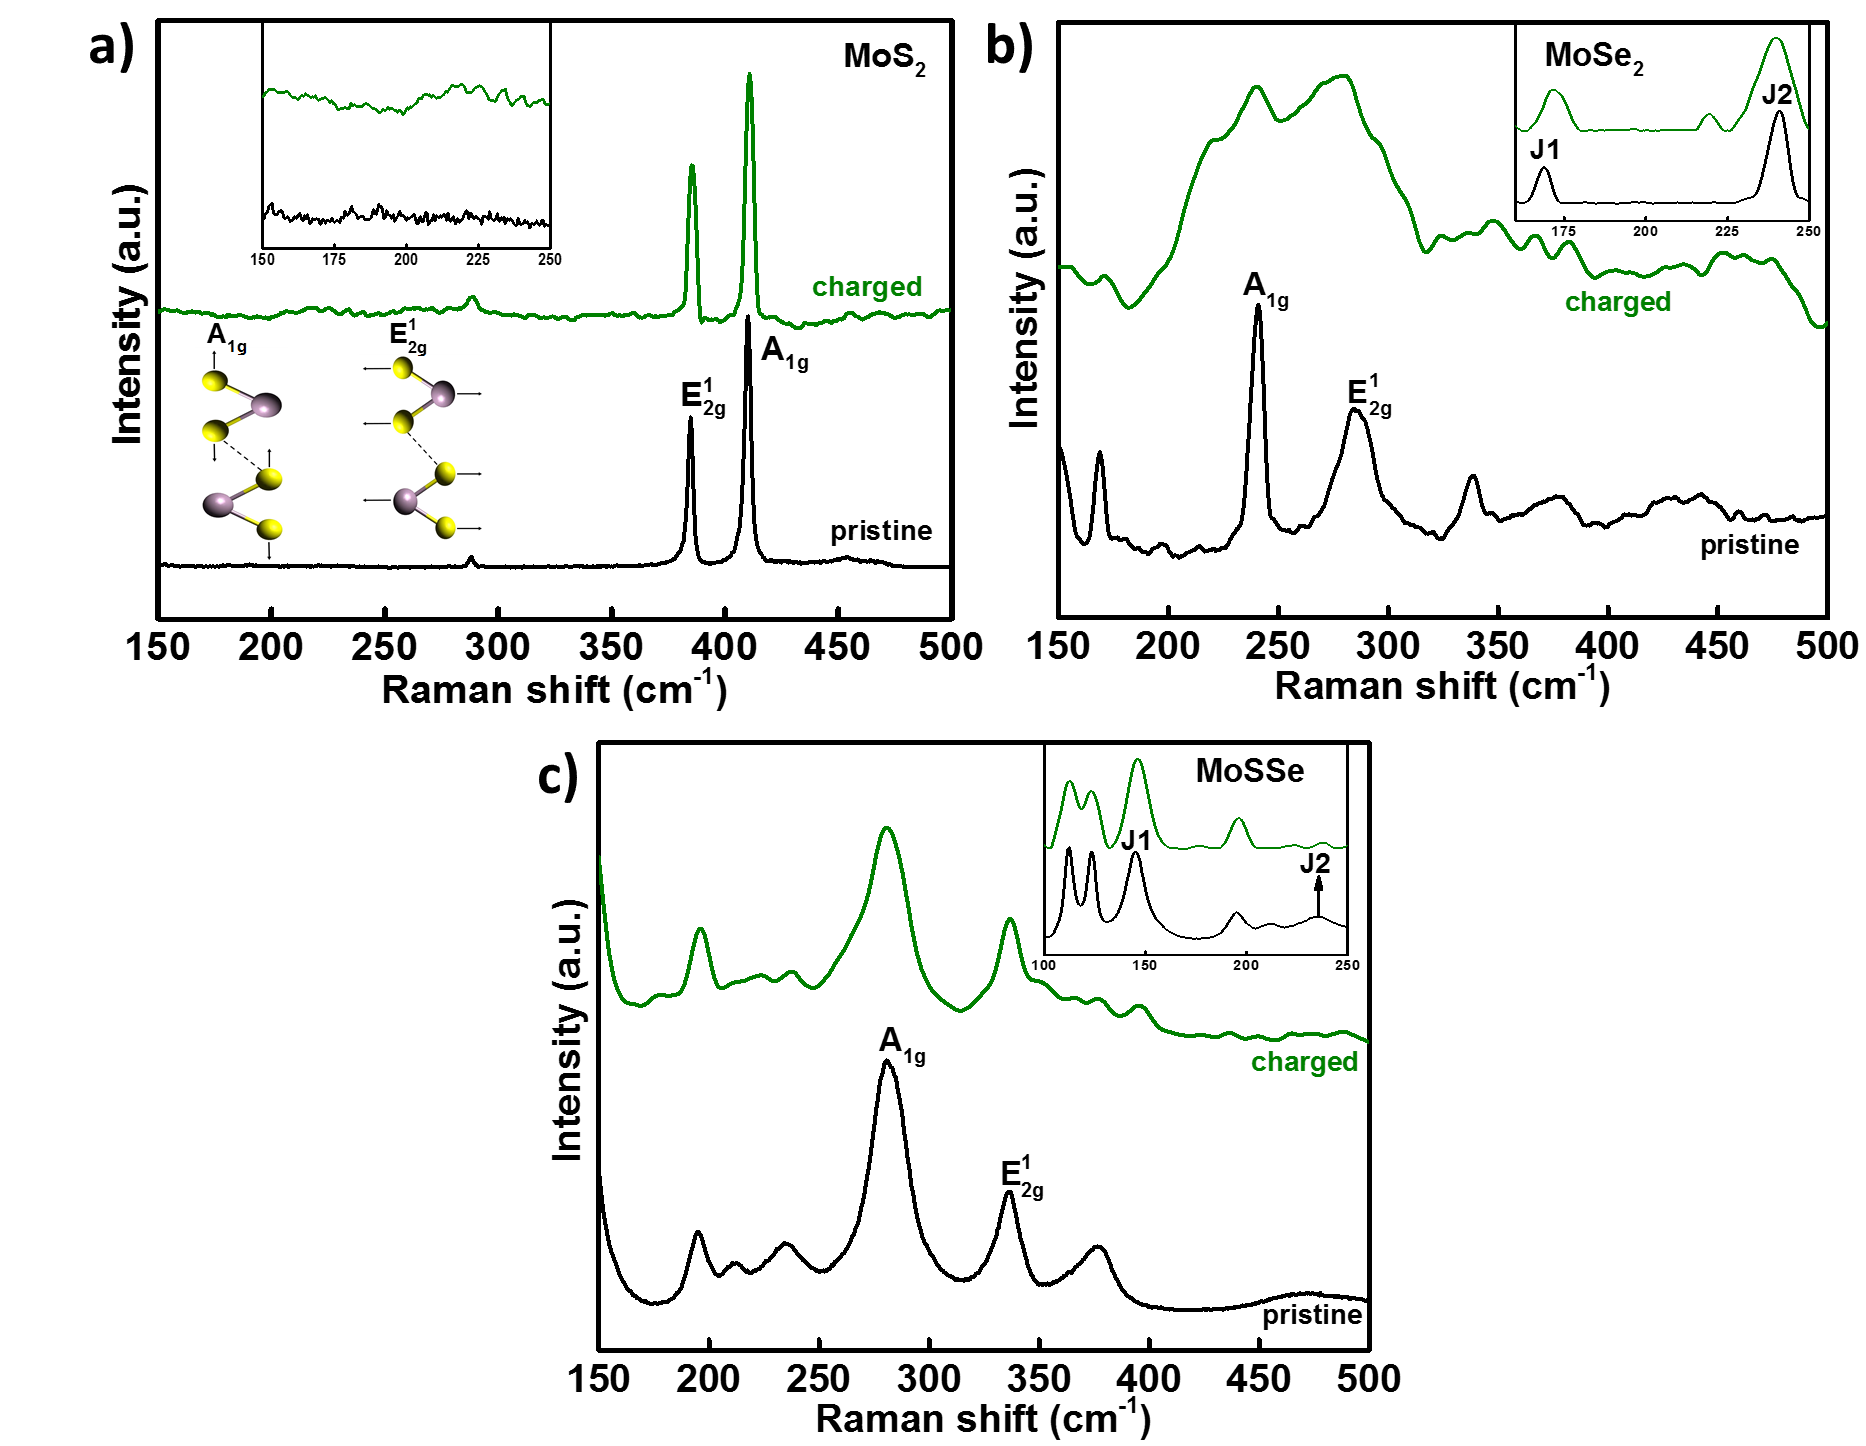
\includegraphics[width=\textwidth]{Figures/chap4fig/raman}
\caption{Raman spectra of pristine (black) and charged (green) a)\ce{MoS2}, b) \ce{MoSe2} and c) MoSSe electrodes with position of new Raman active J1 and J2 bands marked along with E$^1_{2g}$ and A$^1_g$ bands. These bands are however, absent in \ce{MoS2} suggesting no phase change, which correspond to our XRD findings.}
\label{Figures/chap4fig:raman}
\end{figure}
\section{Conclusions}
In summary, \ce{MoSe2} showed a higher capacity and cyclic stability than \ce{MoS2} and MoSSe, as a cathode material for AIBs. CV and XPS results indicated an irreversible phase transition from 2H to the more metallic 1T phase. Our XRD, XPS and Raman results support the hypothesis that \ce{AlCl4-} intercalated reversibly into \ce{MoSe2} with formation of a new complex. A DFT analysis is crucial to determine the nature of this complex. Reversible intercalation of ions along with an additional electro-capacitive behaviour, resulted in a better performance of \ce{MoSe2} electrodes. The cell had a high average voltage of $\sim$2.0 V, and it delivered a specific capacity of about 80 mAh g$^{-1}$ with nearly 95\%\ coulombic efficiency at a current density of 40 mA g$^{-1}$. Our future work would be based on exfoliation of these bulk materials, which would definitely improve the battery performance. 

\newcommand{\beginsupplement}{
               \setcounter{figure}{0}
        \renewcommand{\thefigure}{S\arabic{figure}}
     }
\beginsupplement
\begin{figure}[htb!]
\centering
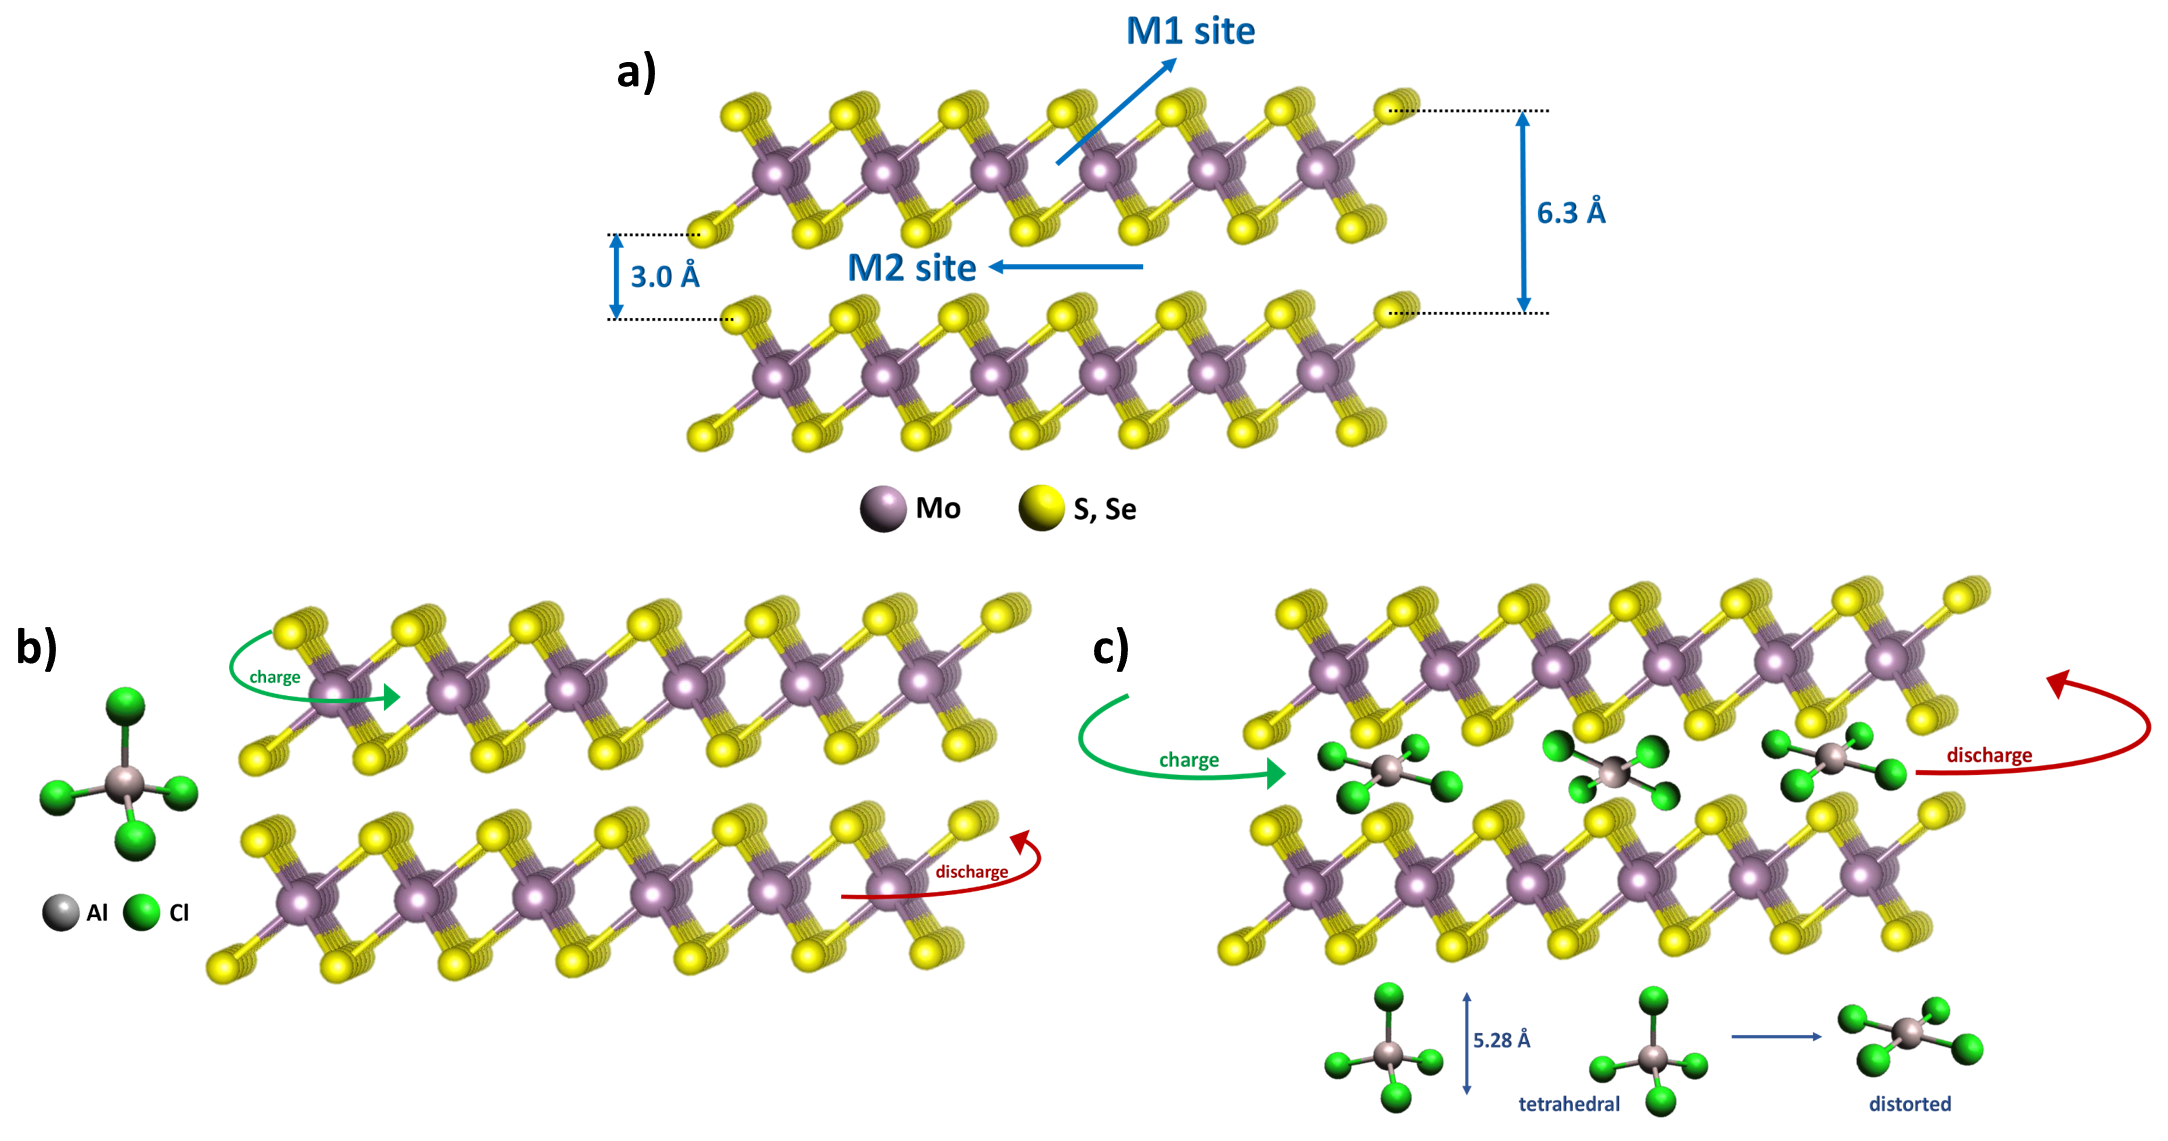
\includegraphics[width=\textwidth]{Figures/chap4fig/S1}
\caption{Galvanostatic charge/discharge profile of the first three cycles of a) \ce{MoS2}, b) \ce{MoSe2} and c) MoSSe at a current rate of 40 mA g$^{-1}$ in a two-electrode setup.}
\label{Figures/chap4fig:S1}
\end{figure}
\begin{figure}[htb!]
\centering
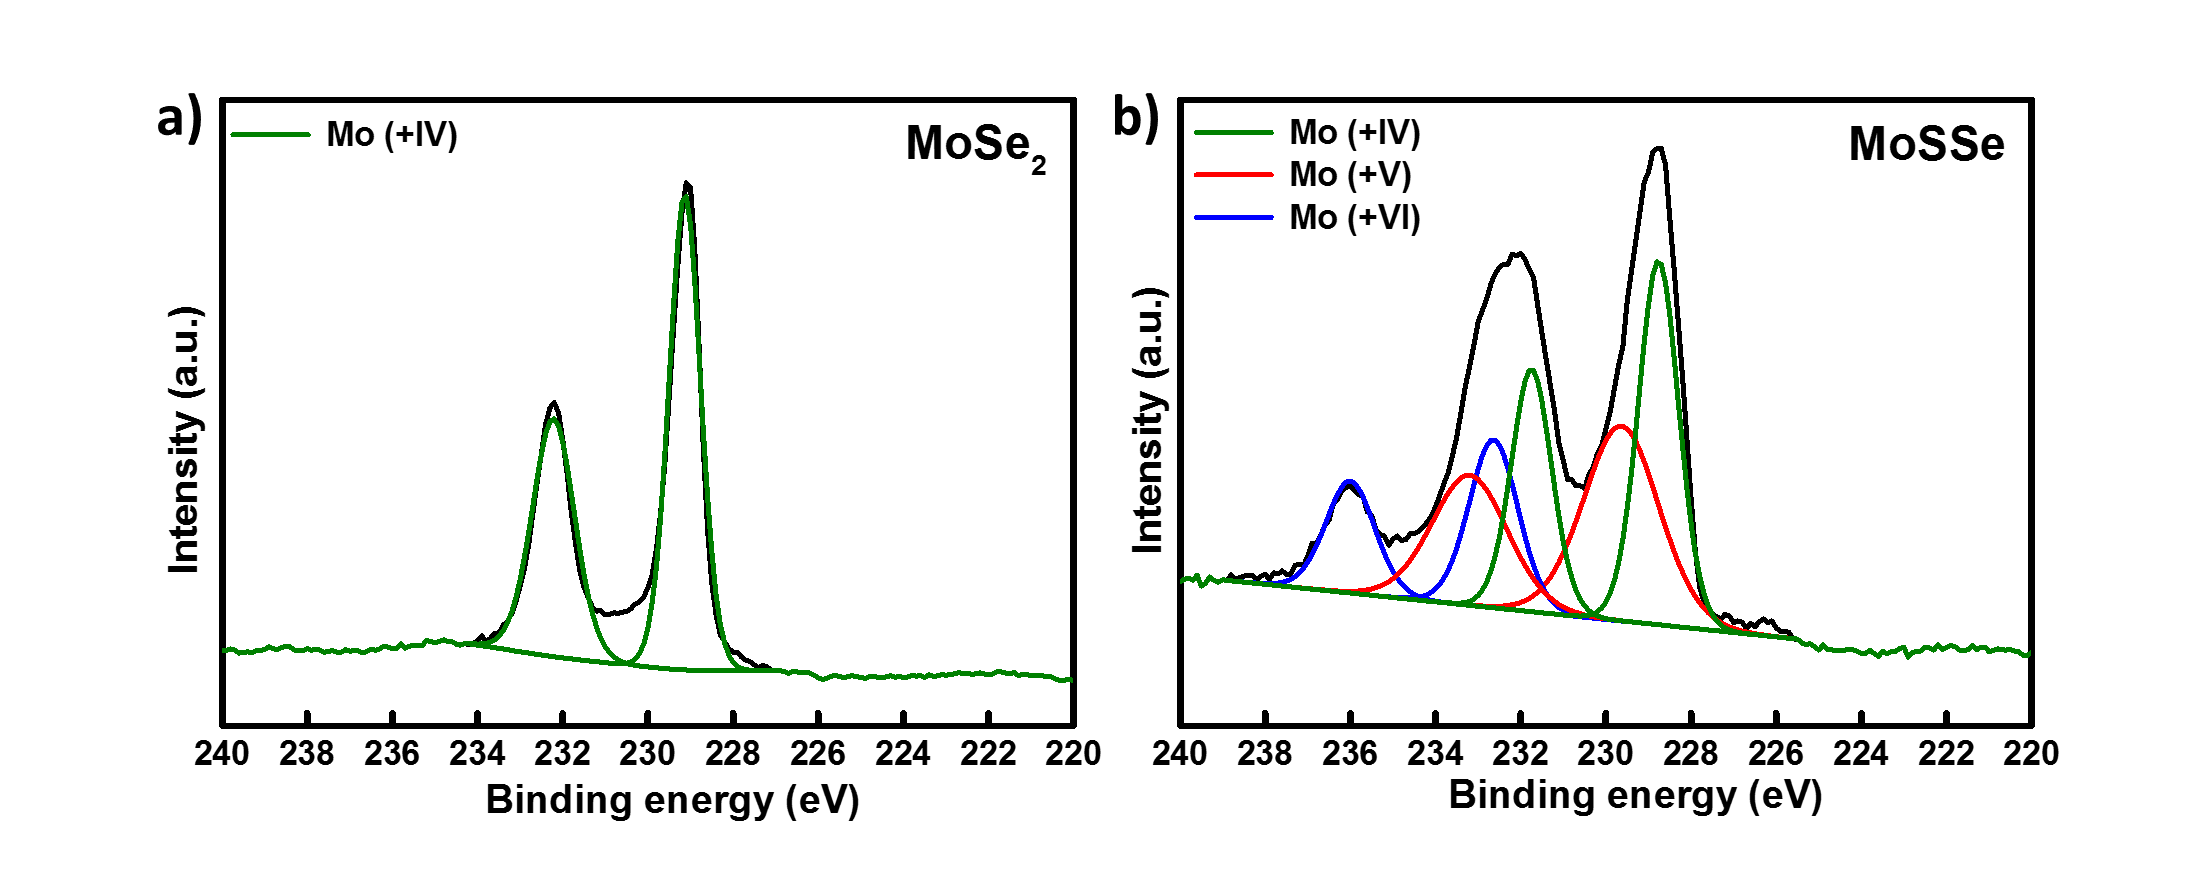
\includegraphics[width=\textwidth]{Figures/chap4fig/S3}
\caption{XPS spectra of Mo 3d for pristine a) \ce{MoSe2} and b) MoSSe electrodes. For \ce{MoSe2}, molybdenum observed its pristine peaks at binding energies at 232.2 eV and 229.1 eV depicting \ce{Mo^{4+}} from \ce{MoSe2}. The Mo peaks in pristine MoSSe electrode observed a complicated spectra. Three doublet peaks appeared corresponding to various oxidation states  and \ce{Mo^{6+}} with 2H and 1T polymorphs already present. }
\label{Figures/chap4fig:S3}
\end{figure}
\begin{figure}[htb!]
\centering
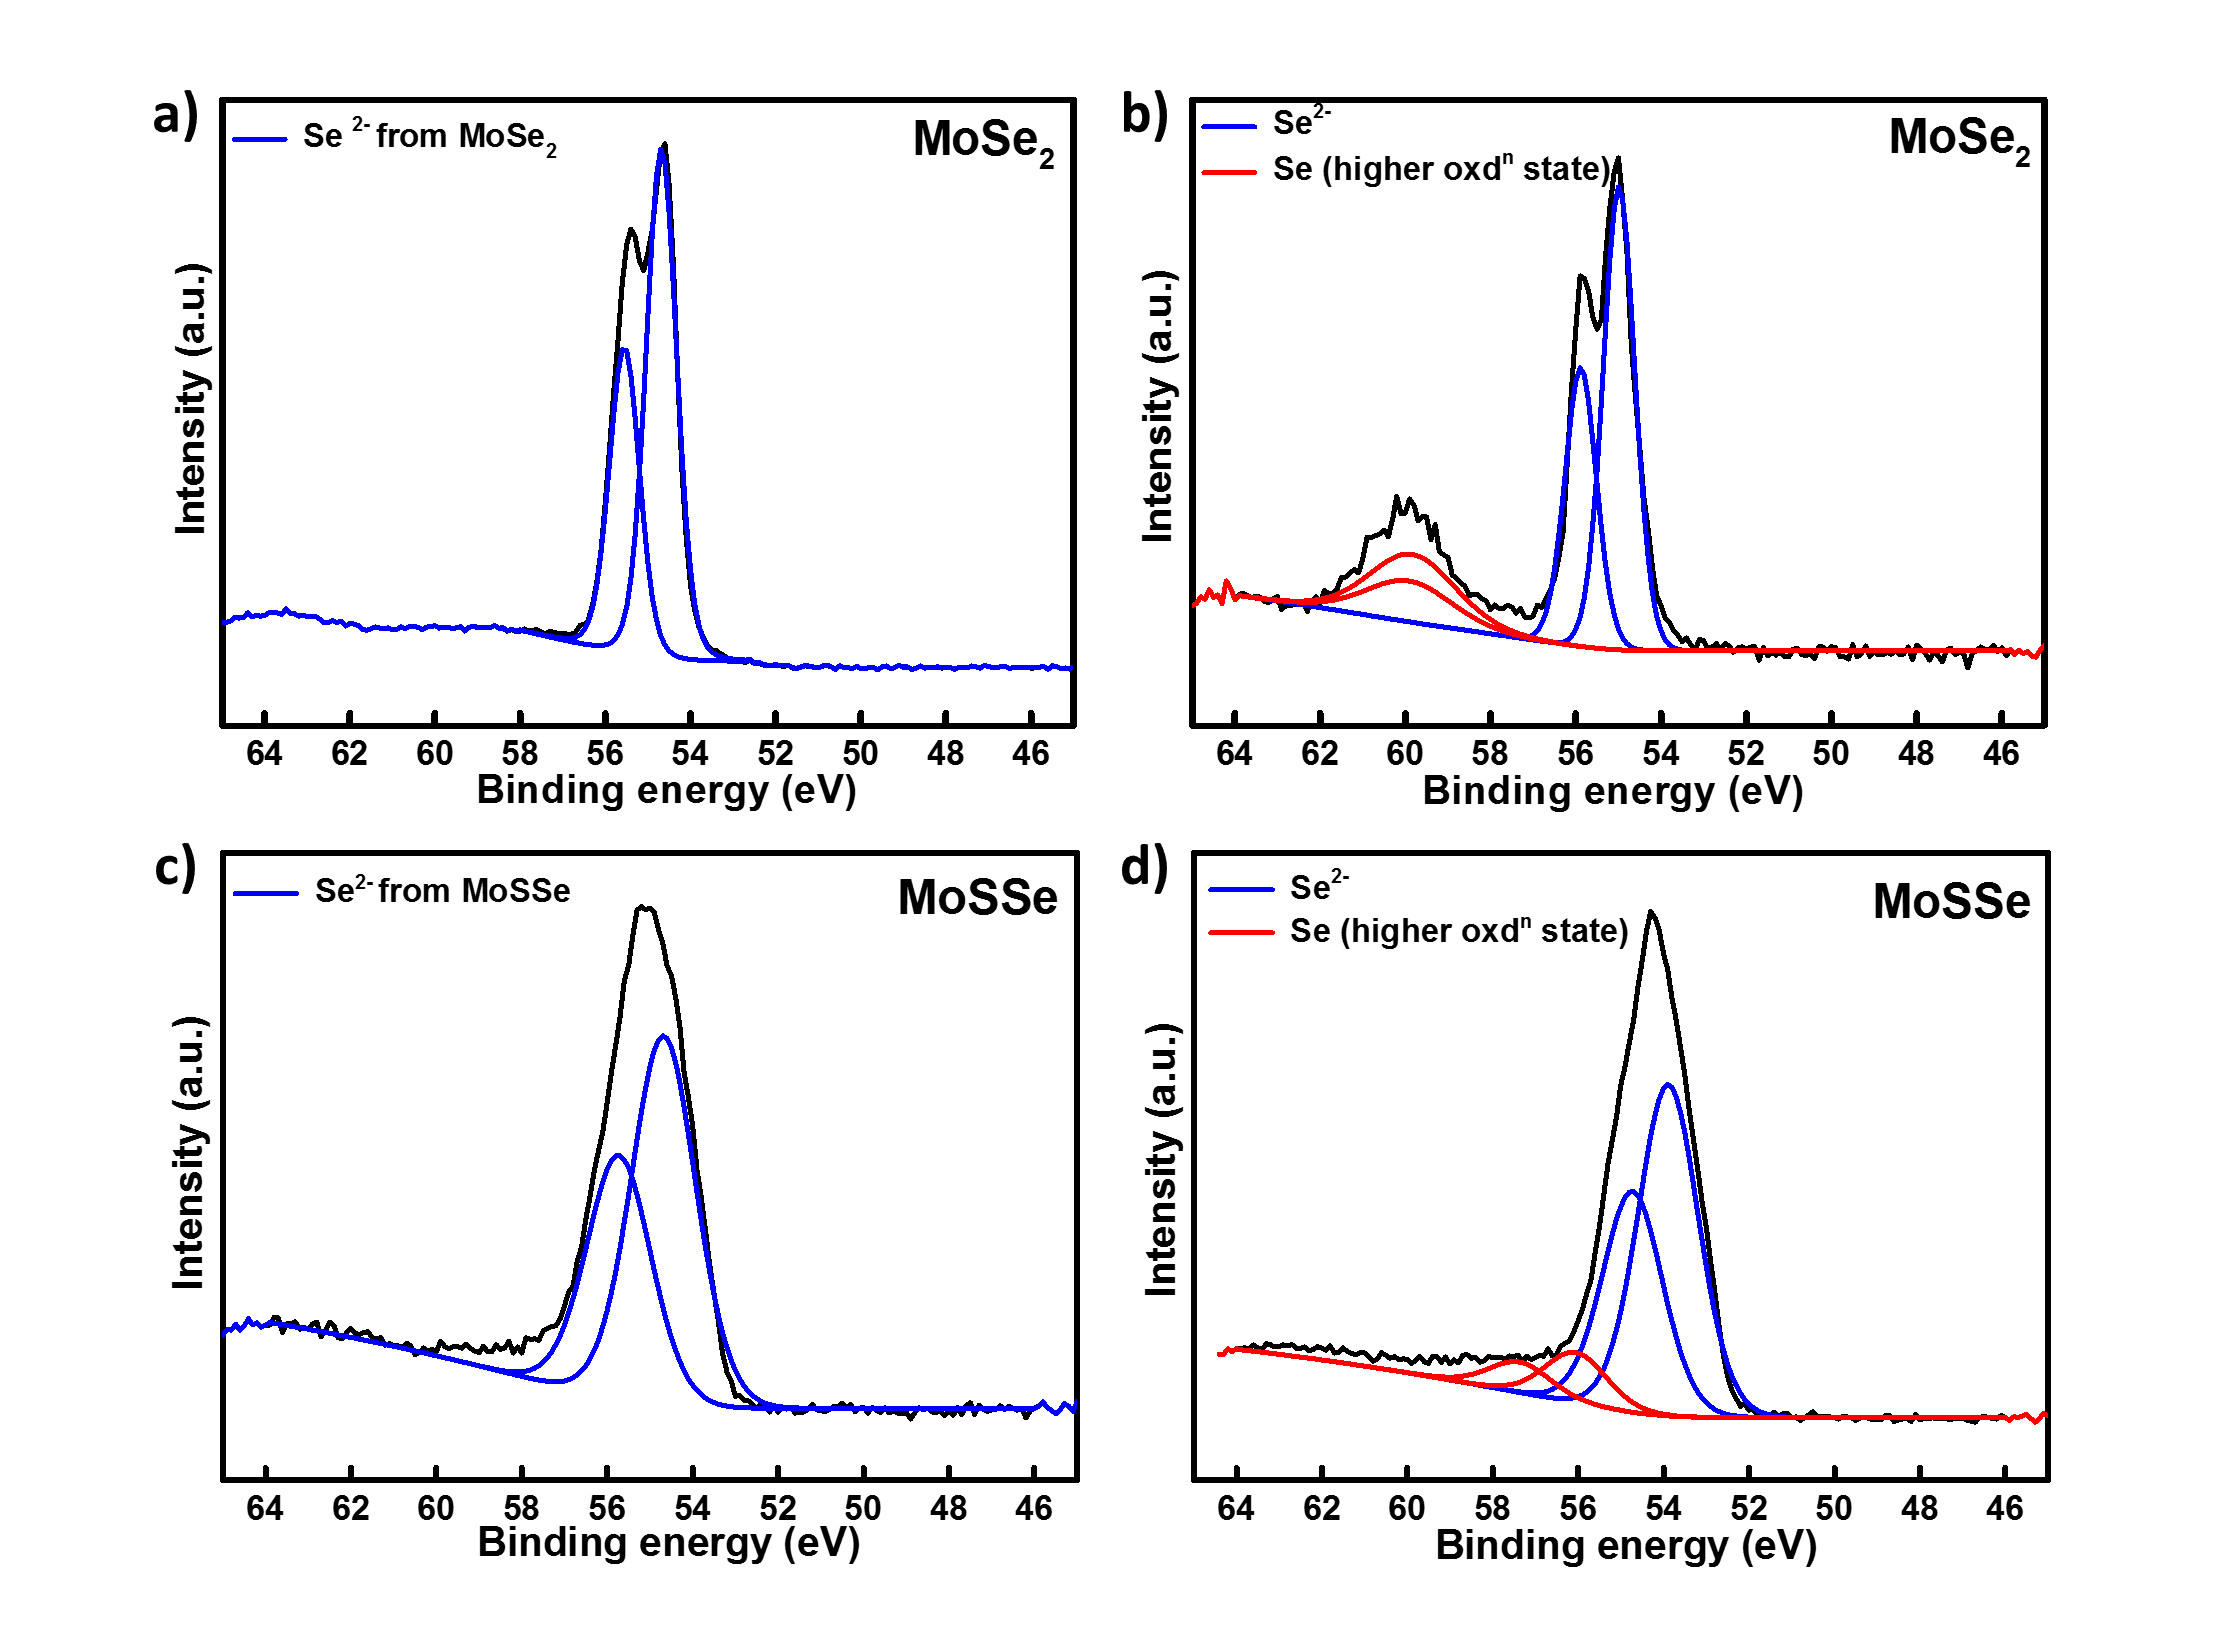
\includegraphics[width=\textwidth]{Figures/chap4fig/S4}
\caption{XPS spectra of Selenium 3d from a) pristine and b) charged electrodes of Al/\ce{MoSe2} cell. Pristine electrode from \ce{MoSe2} observed the characteristic peaks at 55.6 eV and 54.6 eV corresponding to 3d$_{3/2}$ and 3d$_{5/2}$ respectively. After charge, a new peak appeared at 60 eV. We assume this peak arises from a complex (Al$_X$Cl$_y$.\ce{MoSe2}), which forms when \ce{AlCl4-} intercalate into \ce{MoSe2} layers. XPS spectra of Selenium 3d from c) pristine and d) charged electrodes of Al/MoSSe cell.Selenium observed a new doublet after charge.}
\label{Figures/chap4fig:S4}
\end{figure}
\begin{figure}[htb!]
\centering
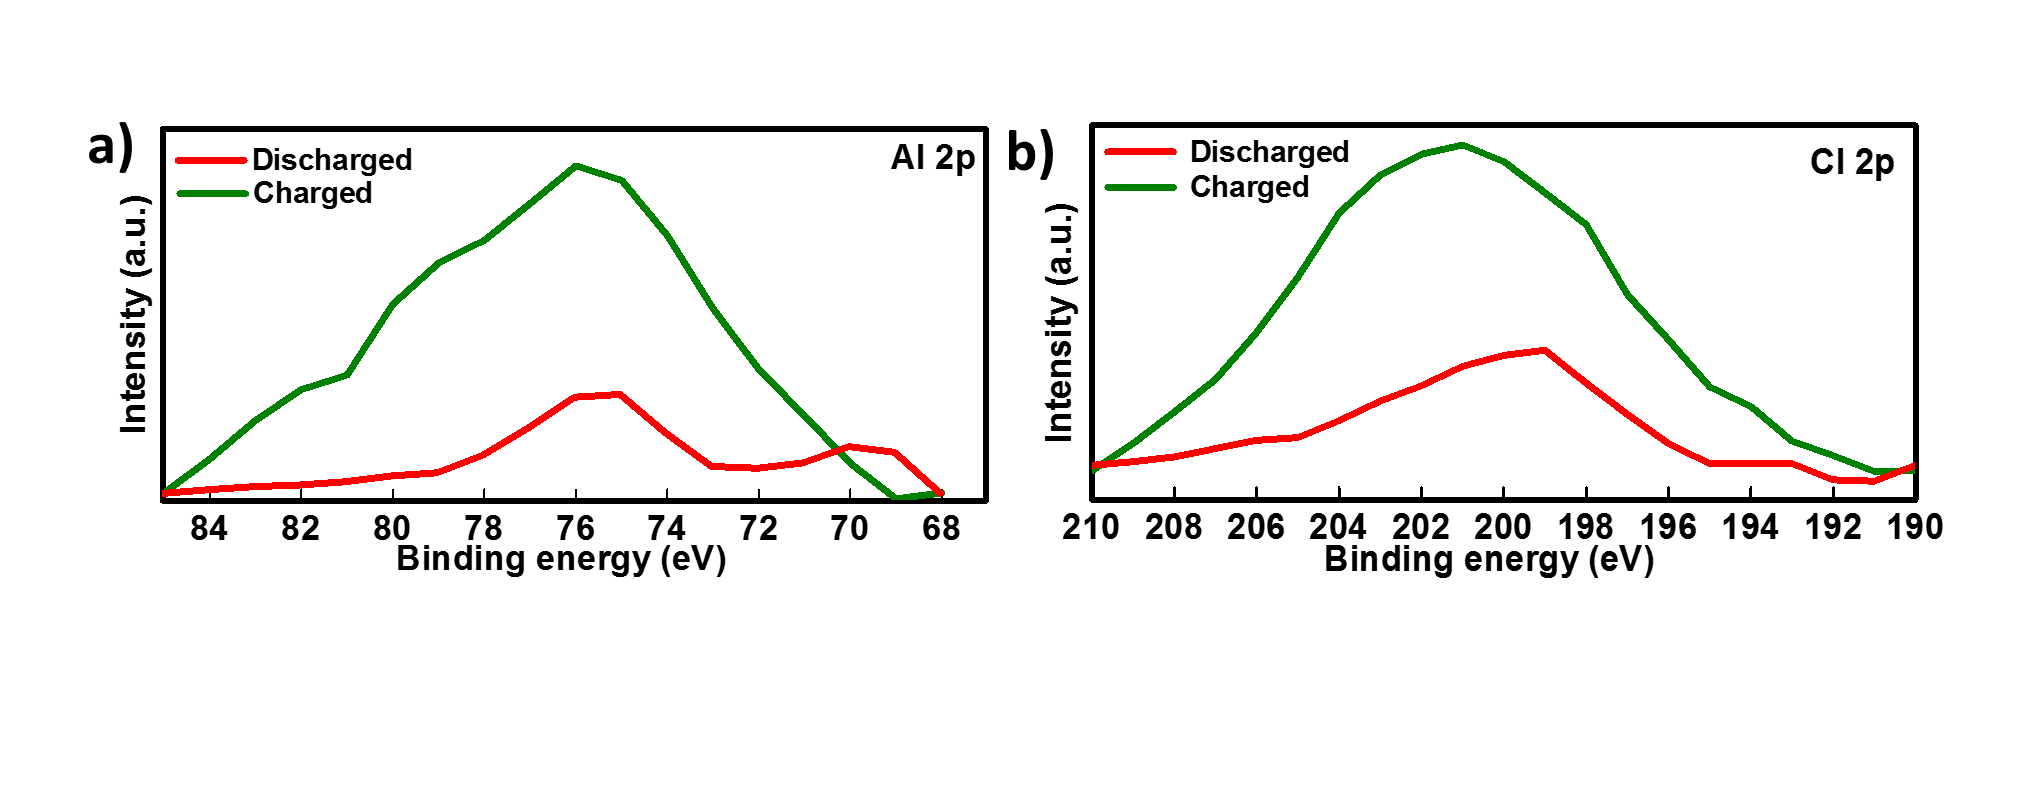
\includegraphics[width=\textwidth]{Figures/chap4fig/S5}
\caption{General trend followed by \ce{MoX2} XPS spectra for a charged and discharged electrode. A higher concentration of Al 2p and Cl 2p peaks were observed in the charged electrodes suggesting an intercalation of \ce{AlCl4-} ions}
\label{Figures/chap4fig:S5}
\end{figure}
\begin{figure}[htb!]
\centering
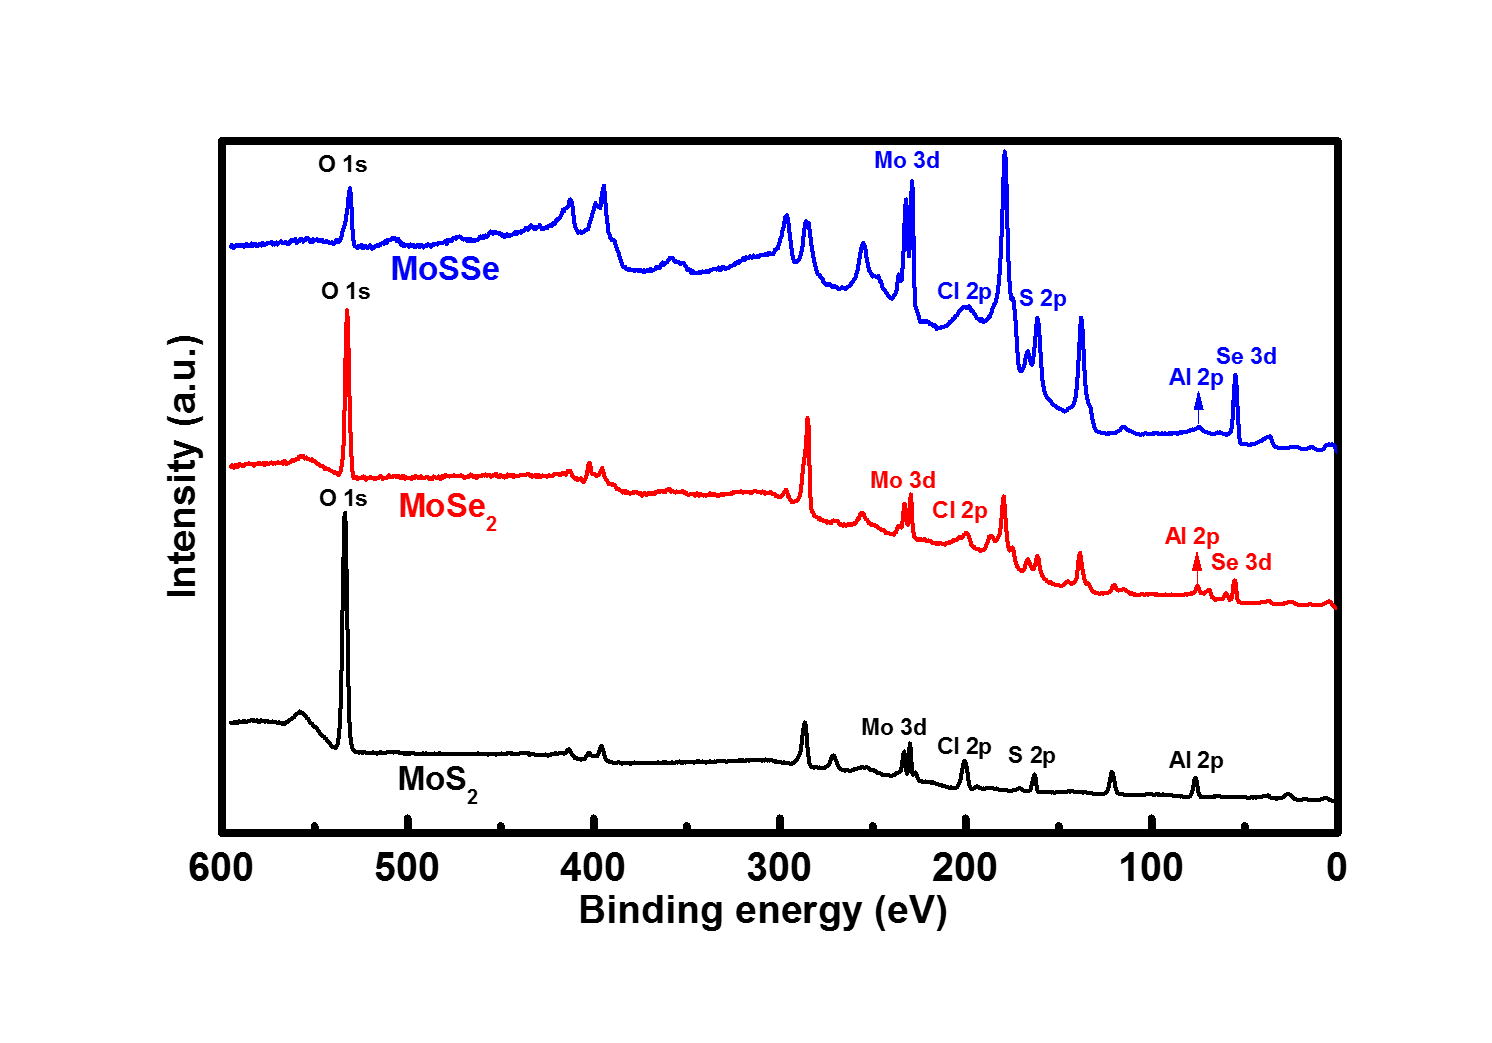
\includegraphics[width=\textwidth]{Figures/chap4fig/S6}
\caption{XPS spectra of a charged \ce{MoS2} (in black), \ce{MoSe2} (in red) and \ce{MoSSe} (in blue) showing characteristic peaks of Mo 3d, S 2p and Se 3d along with presence of Al 2p and Cl 2p.}
\label{Figures/chap4fig:S6}
\end{figure}
\begin{figure}[htb!]
\centering
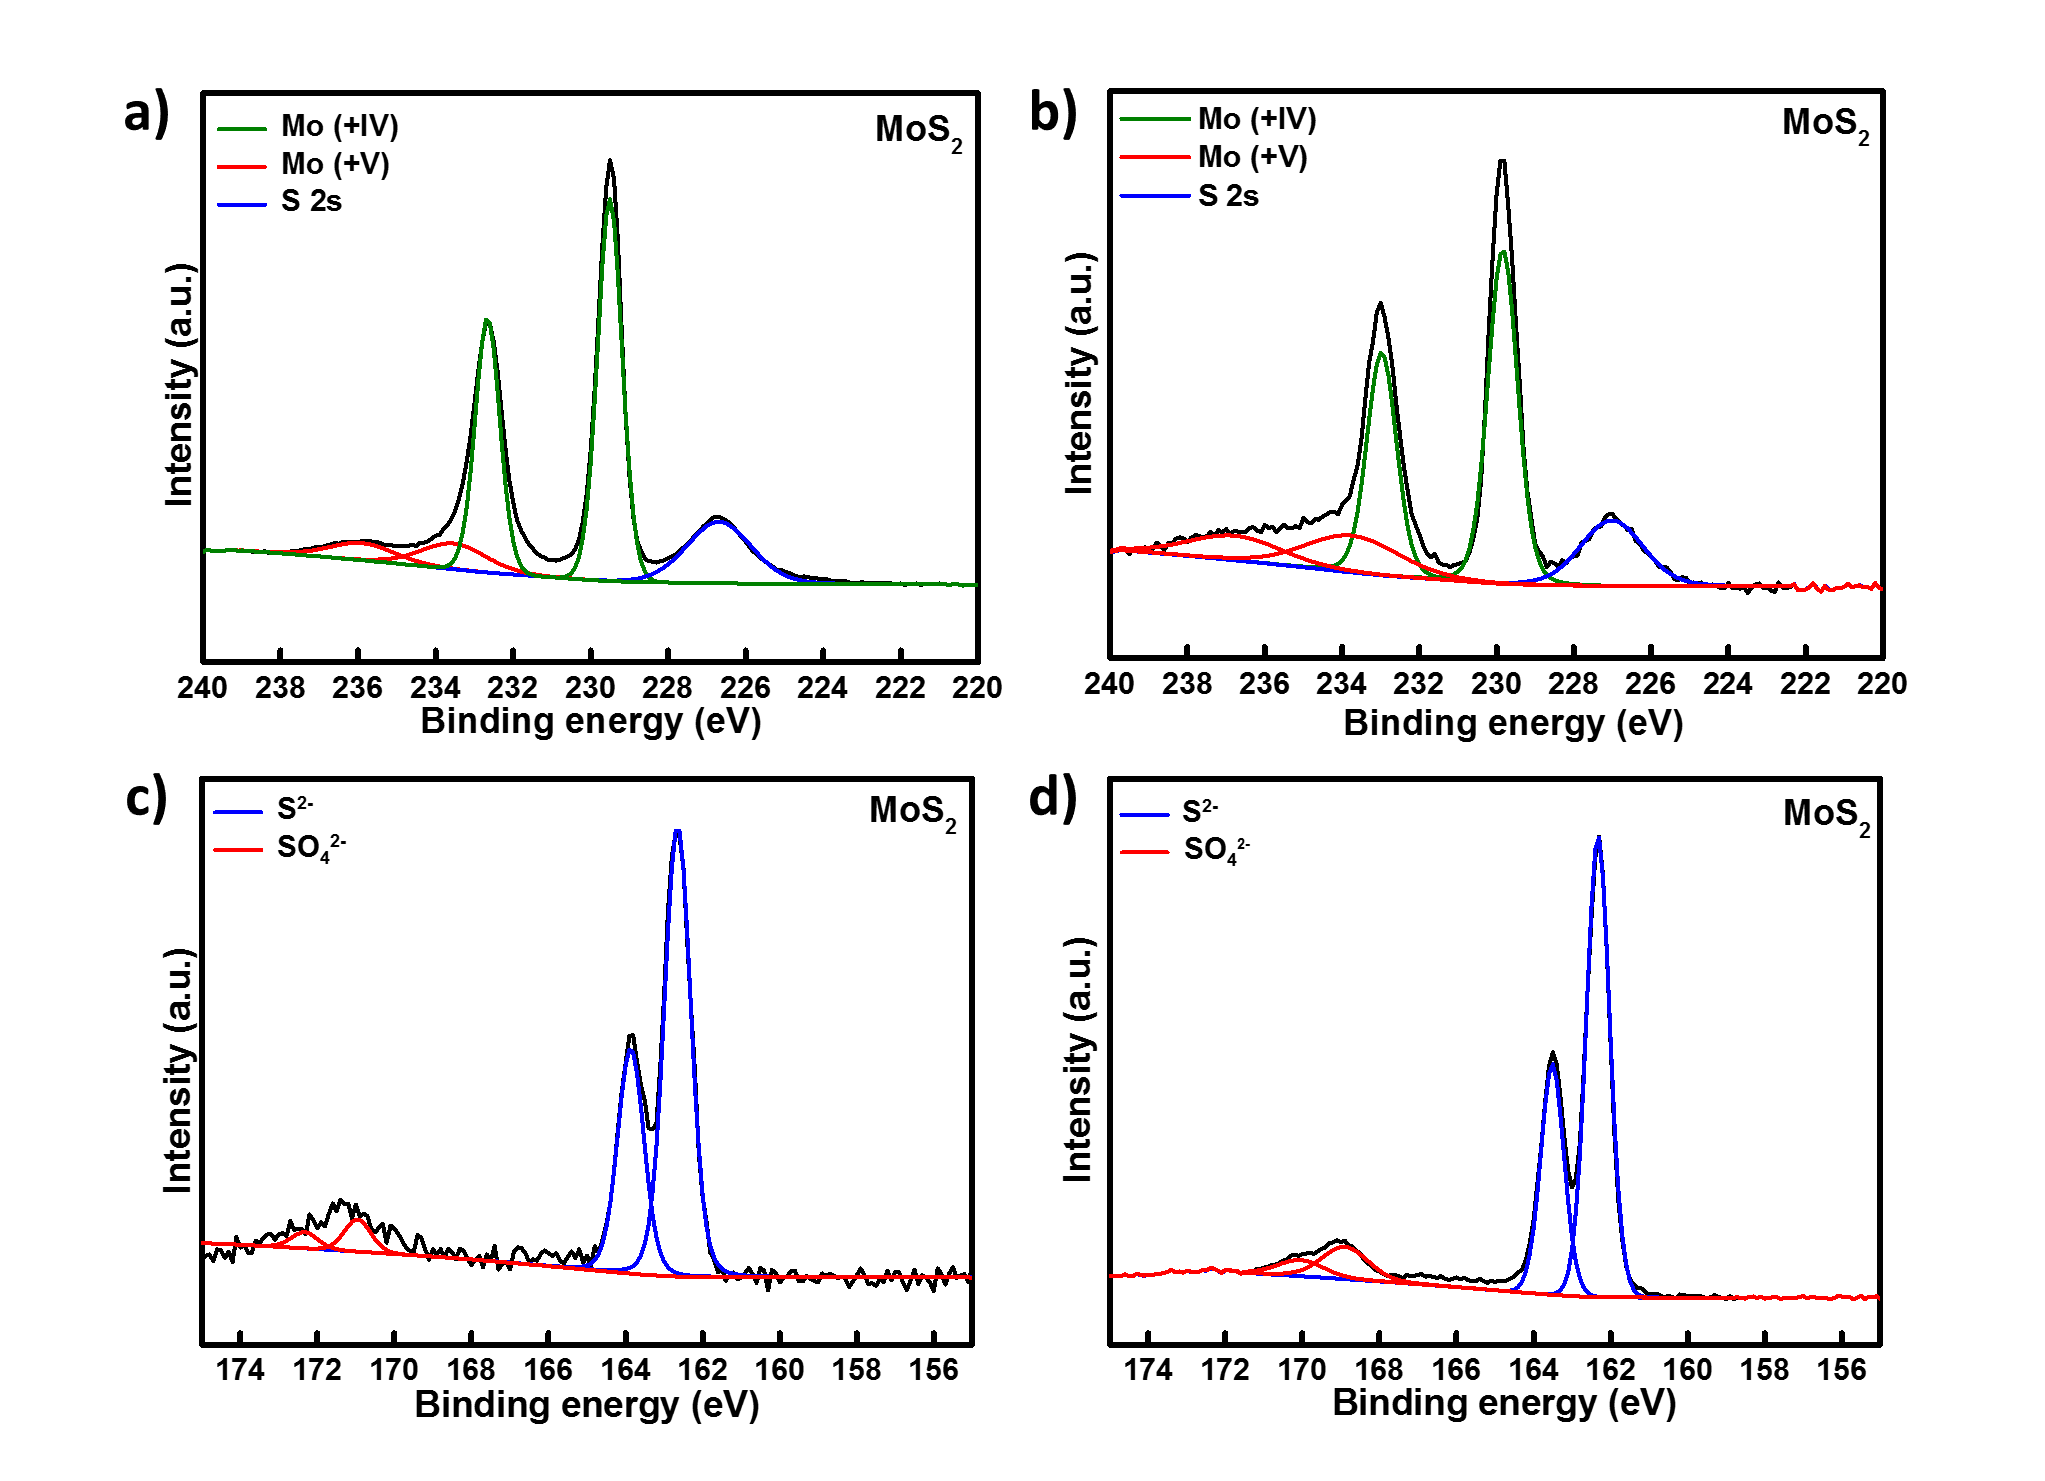
\includegraphics[width=\textwidth]{Figures/chap4fig/S7}
\caption{XPS spectra of Molybdenum 3d for a) pristine and b) charged \ce{MoS2} electrodes. It was noted that after charge, the quantity of high oxidation state Mo (in red) increased. The chemical environment of Mo atoms change after interaction with chloroaluminates which might be due to formation of an intermediate complex (Al$_x$Cl$_y$.\ce{MoS2}). The blue peak at 226 eV indicates the 2s peak for Sulfur. \\XPS spectra of S 2p for c) pristine and d) charged \ce{MoS2} electrodes.}
\label{Figures/chap4fig:S7}
\end{figure}

\begin{figure}[htb!]
\centering

\includegraphics[width=8cm]{Figures/chap4fig/S8}
\caption{Electrochemical performance of a blank molybdenum foil. This shows that the capacity of the cell comes solely from the active material.}
\label{Figures/chap4fig:S8}
\end{figure}
\section{Conclusion and future outlook}


